% Options for packages loaded elsewhere
\PassOptionsToPackage{unicode}{hyperref}
\PassOptionsToPackage{hyphens}{url}
\PassOptionsToPackage{dvipsnames,svgnames,x11names}{xcolor}
%
\documentclass[
  letterpaper,
  DIV=11,
  numbers=noendperiod]{scrartcl}

\usepackage{amsmath,amssymb}
\usepackage{lmodern}
\usepackage{iftex}
\ifPDFTeX
  \usepackage[T1]{fontenc}
  \usepackage[utf8]{inputenc}
  \usepackage{textcomp} % provide euro and other symbols
\else % if luatex or xetex
  \usepackage{unicode-math}
  \defaultfontfeatures{Scale=MatchLowercase}
  \defaultfontfeatures[\rmfamily]{Ligatures=TeX,Scale=1}
\fi
% Use upquote if available, for straight quotes in verbatim environments
\IfFileExists{upquote.sty}{\usepackage{upquote}}{}
\IfFileExists{microtype.sty}{% use microtype if available
  \usepackage[]{microtype}
  \UseMicrotypeSet[protrusion]{basicmath} % disable protrusion for tt fonts
}{}
\makeatletter
\@ifundefined{KOMAClassName}{% if non-KOMA class
  \IfFileExists{parskip.sty}{%
    \usepackage{parskip}
  }{% else
    \setlength{\parindent}{0pt}
    \setlength{\parskip}{6pt plus 2pt minus 1pt}}
}{% if KOMA class
  \KOMAoptions{parskip=half}}
\makeatother
\usepackage{xcolor}
\setlength{\emergencystretch}{3em} % prevent overfull lines
\setcounter{secnumdepth}{5}
% Make \paragraph and \subparagraph free-standing
\ifx\paragraph\undefined\else
  \let\oldparagraph\paragraph
  \renewcommand{\paragraph}[1]{\oldparagraph{#1}\mbox{}}
\fi
\ifx\subparagraph\undefined\else
  \let\oldsubparagraph\subparagraph
  \renewcommand{\subparagraph}[1]{\oldsubparagraph{#1}\mbox{}}
\fi


\providecommand{\tightlist}{%
  \setlength{\itemsep}{0pt}\setlength{\parskip}{0pt}}\usepackage{longtable,booktabs,array}
\usepackage{calc} % for calculating minipage widths
% Correct order of tables after \paragraph or \subparagraph
\usepackage{etoolbox}
\makeatletter
\patchcmd\longtable{\par}{\if@noskipsec\mbox{}\fi\par}{}{}
\makeatother
% Allow footnotes in longtable head/foot
\IfFileExists{footnotehyper.sty}{\usepackage{footnotehyper}}{\usepackage{footnote}}
\makesavenoteenv{longtable}
\usepackage{graphicx}
\makeatletter
\def\maxwidth{\ifdim\Gin@nat@width>\linewidth\linewidth\else\Gin@nat@width\fi}
\def\maxheight{\ifdim\Gin@nat@height>\textheight\textheight\else\Gin@nat@height\fi}
\makeatother
% Scale images if necessary, so that they will not overflow the page
% margins by default, and it is still possible to overwrite the defaults
% using explicit options in \includegraphics[width, height, ...]{}
\setkeys{Gin}{width=\maxwidth,height=\maxheight,keepaspectratio}
% Set default figure placement to htbp
\makeatletter
\def\fps@figure{htbp}
\makeatother
\newlength{\cslhangindent}
\setlength{\cslhangindent}{1.5em}
\newlength{\csllabelwidth}
\setlength{\csllabelwidth}{3em}
\newlength{\cslentryspacingunit} % times entry-spacing
\setlength{\cslentryspacingunit}{\parskip}
\newenvironment{CSLReferences}[2] % #1 hanging-ident, #2 entry spacing
 {% don't indent paragraphs
  \setlength{\parindent}{0pt}
  % turn on hanging indent if param 1 is 1
  \ifodd #1
  \let\oldpar\par
  \def\par{\hangindent=\cslhangindent\oldpar}
  \fi
  % set entry spacing
  \setlength{\parskip}{#2\cslentryspacingunit}
 }%
 {}
\usepackage{calc}
\newcommand{\CSLBlock}[1]{#1\hfill\break}
\newcommand{\CSLLeftMargin}[1]{\parbox[t]{\csllabelwidth}{#1}}
\newcommand{\CSLRightInline}[1]{\parbox[t]{\linewidth - \csllabelwidth}{#1}\break}
\newcommand{\CSLIndent}[1]{\hspace{\cslhangindent}#1}

\KOMAoption{captions}{tableheading}
\makeatletter
\@ifpackageloaded{tcolorbox}{}{\usepackage[many]{tcolorbox}}
\@ifpackageloaded{fontawesome5}{}{\usepackage{fontawesome5}}
\definecolor{quarto-callout-color}{HTML}{909090}
\definecolor{quarto-callout-note-color}{HTML}{0758E5}
\definecolor{quarto-callout-important-color}{HTML}{CC1914}
\definecolor{quarto-callout-warning-color}{HTML}{EB9113}
\definecolor{quarto-callout-tip-color}{HTML}{00A047}
\definecolor{quarto-callout-caution-color}{HTML}{FC5300}
\definecolor{quarto-callout-color-frame}{HTML}{acacac}
\definecolor{quarto-callout-note-color-frame}{HTML}{4582ec}
\definecolor{quarto-callout-important-color-frame}{HTML}{d9534f}
\definecolor{quarto-callout-warning-color-frame}{HTML}{f0ad4e}
\definecolor{quarto-callout-tip-color-frame}{HTML}{02b875}
\definecolor{quarto-callout-caution-color-frame}{HTML}{fd7e14}
\makeatother
\makeatletter
\makeatother
\makeatletter
\makeatother
\makeatletter
\@ifpackageloaded{caption}{}{\usepackage{caption}}
\AtBeginDocument{%
\ifdefined\contentsname
  \renewcommand*\contentsname{Table of contents}
\else
  \newcommand\contentsname{Table of contents}
\fi
\ifdefined\listfigurename
  \renewcommand*\listfigurename{List of Figures}
\else
  \newcommand\listfigurename{List of Figures}
\fi
\ifdefined\listtablename
  \renewcommand*\listtablename{List of Tables}
\else
  \newcommand\listtablename{List of Tables}
\fi
\ifdefined\figurename
  \renewcommand*\figurename{Figure}
\else
  \newcommand\figurename{Figure}
\fi
\ifdefined\tablename
  \renewcommand*\tablename{Table}
\else
  \newcommand\tablename{Table}
\fi
}
\@ifpackageloaded{float}{}{\usepackage{float}}
\floatstyle{ruled}
\@ifundefined{c@chapter}{\newfloat{codelisting}{h}{lop}}{\newfloat{codelisting}{h}{lop}[chapter]}
\floatname{codelisting}{Listing}
\newcommand*\listoflistings{\listof{codelisting}{List of Listings}}
\makeatother
\makeatletter
\@ifpackageloaded{caption}{}{\usepackage{caption}}
\@ifpackageloaded{subcaption}{}{\usepackage{subcaption}}
\makeatother
\makeatletter
\@ifpackageloaded{tcolorbox}{}{\usepackage[many]{tcolorbox}}
\makeatother
\makeatletter
\@ifundefined{shadecolor}{\definecolor{shadecolor}{rgb}{.97, .97, .97}}
\makeatother
\makeatletter
\makeatother
\ifLuaTeX
  \usepackage{selnolig}  % disable illegal ligatures
\fi
\IfFileExists{bookmark.sty}{\usepackage{bookmark}}{\usepackage{hyperref}}
\IfFileExists{xurl.sty}{\usepackage{xurl}}{} % add URL line breaks if available
\urlstyle{same} % disable monospaced font for URLs
% Make links footnotes instead of hotlinks:
\DeclareRobustCommand{\href}[2]{#2\footnote{\url{#1}}}
\hypersetup{
  pdftitle={KIN 377: Motor Learning},
  colorlinks=true,
  linkcolor={blue},
  filecolor={Maroon},
  citecolor={Blue},
  urlcolor={Blue},
  pdfcreator={LaTeX via pandoc}}

\title{KIN 377: Motor Learning}
\usepackage{etoolbox}
\makeatletter
\providecommand{\subtitle}[1]{% add subtitle to \maketitle
  \apptocmd{\@title}{\par {\large #1 \par}}{}{}
}
\makeatother
\subtitle{Department of Kinesiology, Cal State Northridge\\
Syllabus - Spring 2023 (Online and Hybrid)}
\author{}
\date{}

\begin{document}
\maketitle
\ifdefined\Shaded\renewenvironment{Shaded}{\begin{tcolorbox}[enhanced, breakable, boxrule=0pt, borderline west={3pt}{0pt}{shadecolor}, frame hidden, interior hidden, sharp corners]}{\end{tcolorbox}}\fi

\renewcommand*\contentsname{Table of contents}
{
\hypersetup{linkcolor=}
\setcounter{tocdepth}{3}
\tableofcontents
}
\begin{center}\rule{0.5\linewidth}{0.5pt}\end{center}

\href{syllabus.pdf}{Syllabus in PDF format}

\hypertarget{sec-instructor-info}{%
\section{Instructor Info}\label{sec-instructor-info}}

\hypertarget{brief-bio}{%
\subsection{Brief Bio}\label{brief-bio}}

Ovande Furtado Jr., Ph.D.

Dr.~Furtado received a B.A. in Physical Education from the Federal
University of Parana, Curitiba, PR - Brazil. He earned his M.S. and
Ph.D.~degrees in Motor Behavior from the University of Pittsburgh, PA.
Dr.~Furtado's line of research focuses on two main areas: (1) validation
of observational models in psychomotor assessment instruments and (2)
the relationship between motor skill competence, perceived motor
competence, physical activity levels, and body composition.

\hypertarget{office-hours}{%
\subsection{Office Hours}\label{office-hours}}

See Section~\ref{sec-office-hours} for more information

\hypertarget{contact-info}{%
\subsection{Contact Info}\label{contact-info}}

Email: ovandef@csun.edu\\
Office: Redwood Hall 289\\
Course's Site: \url{https://drfurtado.github.io/site/courses/377/}

\begin{tcolorbox}[enhanced jigsaw, leftrule=.75mm, breakable, opacityback=0, bottomrule=.15mm, rightrule=.15mm, colbacktitle=quarto-callout-note-color!10!white, colframe=quarto-callout-note-color-frame, arc=.35mm, bottomtitle=1mm, left=2mm, title=\textcolor{quarto-callout-note-color}{\faInfo}\hspace{0.5em}{Note}, titlerule=0mm, toptitle=1mm, toprule=.15mm, opacitybacktitle=0.6, colback=white, coltitle=black]

For course-related questions, please use our mailing list. This way,
other students will benefit when I answer your question(s). Refer to
Canvas for the mailing list email address.

Hint: Add the email to your contacts for easy access throughout the
semester.

\end{tcolorbox}

\hypertarget{general-information}{%
\section{General Information}\label{general-information}}

\hypertarget{course-description}{%
\subsection{Course Description}\label{course-description}}

Study of principles , theories, and research evidence regarding the
nature of motor performance and learning with particular emphasis on
factors that impact learning a skill through practice.

\begin{itemize}
\tightlist
\item
  teaching
\item
  examples of principles
\item
  educational and clinical settings
\item
  include both catalog and my own description
\item
  do the same with the other items from the excel file
\end{itemize}

\hypertarget{course-prerequisite}{%
\subsection{Course Prerequisite}\label{course-prerequisite}}

\href{https://catalog.csun.edu/academics/kin/courses/kin-200/}{KIN 200}:
Foundations of Kinesiology (3)

\hypertarget{course-format}{%
\subsection{Course Format}\label{course-format}}

This course consists of readings, written assignments, weekly responses,
and check-ins on our Canvas page.

I teach two modes of KIN 377, hybrid and online.

\hypertarget{hybrid-sections}{%
\subsubsection{Hybrid Sections}\label{hybrid-sections}}

A Hybrid class (OH) in which students attend class sessions on campus
and in an online environment. The class typically meets approximately
half online and half on campus.

\begin{itemize}
\tightlist
\item
  \textbf{KIN 377 MOTOR LEARNING - (19392-SP2023)}
\end{itemize}

\hypertarget{online-sections}{%
\subsubsection{Online Sections}\label{online-sections}}

A fully Online class (OF) in which all class sessions and exams are
presented in an online environment; OF courses have no on-campus
meetings.

\begin{itemize}
\item
  \textbf{KIN 377 MOTOR LEARNING - (19430-SP2023)}
\item
  \textbf{KIN 377 MOTOR LEARNING - (19780-SP2023)}
\end{itemize}

\begin{tcolorbox}[enhanced jigsaw, leftrule=.75mm, breakable, opacityback=0, bottomrule=.15mm, rightrule=.15mm, colbacktitle=quarto-callout-warning-color!10!white, colframe=quarto-callout-warning-color-frame, arc=.35mm, bottomtitle=1mm, left=2mm, title=\textcolor{quarto-callout-warning-color}{\faExclamationTriangle}\hspace{0.5em}{Warning}, titlerule=0mm, toptitle=1mm, toprule=.15mm, opacitybacktitle=0.6, colback=white, coltitle=black]

This course is not self-paced and is not the ``softer, easier way''!
This means that you have to \textbf{1) check in regularly and 2) respond
to the weekly assignments.}

\end{tcolorbox}

\hypertarget{sec-required-technology-resources}{%
\subsection{Required Technology
Resources}\label{sec-required-technology-resources}}

This course will be taught completely online (no campus meetings will be
required), in an asynchronous format (this course will not have
scheduled live meeting times). All activities, assignments and exams in
this course will be completed via Canvas. To succeed in this course, you
must have reliable access to a computer and internet connection. CSUN
offers currently enrolled students the option to borrow devices such as
computers and internet \texttt{hotspots} through its
\href{https://www.csun.edu/it/device-loaner-program}{Device Loaner
Program}.

\hypertarget{course-expectations-and-goals}{%
\subsection{Course Expectations and
Goals}\label{course-expectations-and-goals}}

At the conclusion of this course, students should be able to:

\begin{enumerate}
\def\labelenumi{\arabic{enumi}.}
\tightlist
\item
  Describe the difference between motor learning and performance.
\item
  Describe and understand different theories of control to explain how
  motor skills are performed and learned.
\item
  Describe and understand the underlying mechanisms and processes
  involved in the production and control of movement.
\item
  Discuss the relationship between attention and performance.
\item
  Understand and demonstrate how factors relevant to the individual and
  to the environment influence the learning process.
\item
  Understand and demonstrate how feedback types and schedules influence
  motor skill learning.
\item
  Understand, describe, and demonstrate how practice schedules influence
  motor skill learning.
\item
  Describe how and why the concept of individual differences is
  important in skill acquisition.

  \begin{enumerate}
  \def\labelenumii{\arabic{enumii}.}
  \tightlist
  \item
    Describe and understand motor learning and control issues for
    special populations.
  \end{enumerate}
\item
  Develop and implement methods of performance assessments.
\item
  Develop and implement a series of practice sessions designed to teach
  and/or learn a novel motor skill.
\end{enumerate}

\hypertarget{student-learning-outcomes-slos}{%
\subsection{Student Learning Outcomes
(SLO'S)}\label{student-learning-outcomes-slos}}

\begin{enumerate}
\def\labelenumi{\arabic{enumi}.}
\tightlist
\item
  Apply an integrated kinesiological approach to encourage the adoption
  of healthy and physically active lifestyles, across diverse
  populations;
\item
  Apply evidence-based practices to enhance the study of human movement;
\item
  Demonstrate competent problem-solving strategies through intentional
  practices; and
\item
  Demonstrate knowledge of kinesthetic forms, processes, and structures
  as they apply to the personal expression and culture of human
  movement.
\end{enumerate}

\hypertarget{textbook}{%
\subsection{Textbook}\label{textbook}}

Magill, R. A., \& Anderson, D. (2020). Motor learning and control:
concepts and applications (12th Ed.). McGraw-Hill Education.

Link to Matador Bookstore: \url{https://bit.ly/37yiD7u}

\begin{tcolorbox}[enhanced jigsaw, leftrule=.75mm, breakable, opacityback=0, bottomrule=.15mm, rightrule=.15mm, colbacktitle=quarto-callout-note-color!10!white, colframe=quarto-callout-note-color-frame, arc=.35mm, bottomtitle=1mm, left=2mm, title=\textcolor{quarto-callout-note-color}{\faInfo}\hspace{0.5em}{Note}, titlerule=0mm, toptitle=1mm, toprule=.15mm, opacitybacktitle=0.6, colback=white, coltitle=black]

The program below is only available during the Fall and Spring
semesters.

\end{tcolorbox}

\hypertarget{sec-mycsundigitalaccess}{%
\subsubsection{myCSUNDigitalAccess
Program}\label{sec-mycsundigitalaccess}}

\begin{enumerate}
\def\labelenumi{\arabic{enumi}.}
\tightlist
\item
  You are enrolled in a course which is part of the myCSUNDigitalAccess
  (MCDA) program.
\item
  The \emph{MCDA} program provides digital materials to students at a
  deeply discounted price.
\item
  Some or all of your materials for this course are being provided
  digitally through the \emph{MCDA} program.
\item
  ALL enrolled students will have access to the materials through Canvas
  by the 1st day of class, \emph{but more likely earlier}.
\item
  If you want to keep access throughout the semester, you need do
  nothing. A charge will be placed on your CSUN student portal account
  (just like tuition, but a separate charge) around the 5th or 6th week
  of classes. You will then be responsible for paying the university.
\item
  If you choose to obtain your materials elsewhere you have until
  \textbf{\texttt{02/17/23}} to Opt-Out (see instructions below). Those
  who Opt-Out by \textbf{\texttt{02/17/23}} will lose access and will
  \textbf{not be charged}.
\item
  Anyone who does not Opt-Out by the \textbf{\texttt{02/17/23}} deadline
  will be charged and those charges \textbf{will not be reversible}.
\item
  \href{https://bit.ly/3pcWcfb}{Click here for more information}.
\end{enumerate}

\hypertarget{price}{%
\subsubsection{Price}\label{price}}

To see how much you will be billed if you opt-in, click the link below:

\url{https://bit.ly/3PDiGCx}

\hypertarget{opt-out-instructions}{%
\subsubsection{Opt-out Instructions}\label{opt-out-instructions}}

If you wish to opt out of this program and not purchase access to the
required digital materials you will need to follow the steps below by
\textbf{\texttt{02/17/23}}:

\begin{enumerate}
\def\labelenumi{\arabic{enumi}.}
\tightlist
\item
  Go to \url{https://accessportal.follett.com/0150}
\item
  Click on Create an Account on the lower right
\item
  Create an account using your CSUN email account
\item
  Select the course(s) you wish to Opt-Out from
\end{enumerate}

\begin{tcolorbox}[enhanced jigsaw, leftrule=.75mm, breakable, opacityback=0, bottomrule=.15mm, rightrule=.15mm, colbacktitle=quarto-callout-note-color!10!white, colframe=quarto-callout-note-color-frame, arc=.35mm, bottomtitle=1mm, left=2mm, title=\textcolor{quarto-callout-note-color}{\faInfo}\hspace{0.5em}{Note}, titlerule=0mm, toptitle=1mm, toprule=.15mm, opacitybacktitle=0.6, colback=white, coltitle=black]

You will receive an email confirming your Opt Out selection, access will
be removed and you will need to purchase the materials elsewhere on your
own. For more information about this program, please visit the following
link: \url{https://bit.ly/3pcWcfb}

\end{tcolorbox}

\hypertarget{additional-resources}{%
\subsection{Additional resources}\label{additional-resources}}

\hypertarget{access-to-computer-internet}{%
\subsubsection{Access to Computer \&
Internet}\label{access-to-computer-internet}}

Although not required, it is suggested that you have access to a
computer (not simply a tablet and/or smartphone) and Internet throughout
this course. Note that CSUN students are eligible to
\href{https://www.csun.edu/it/device-loaner-program}{check out tech
devices from CSUN at NO COST}.

\hypertarget{mini-juggling-balls}{%
\subsubsection{Mini Juggling Balls}\label{mini-juggling-balls}}

One of the requirements of this course is to learn a motor skill. If you
select juggling, I suggest you to acquire the
\href{http://goo.gl/X3EjLE}{mini juggling balls}, which are small and
have the recommended weight for beginners.

\begin{tcolorbox}[enhanced jigsaw, leftrule=.75mm, breakable, opacityback=0, bottomrule=.15mm, rightrule=.15mm, colbacktitle=quarto-callout-important-color!10!white, colframe=quarto-callout-important-color-frame, arc=.35mm, bottomtitle=1mm, left=2mm, title=\textcolor{quarto-callout-important-color}{\faExclamation}\hspace{0.5em}{Important}, titlerule=0mm, toptitle=1mm, toprule=.15mm, opacitybacktitle=0.6, colback=white, coltitle=black]

If you choose to use any object other than the mini juggling balls,
understand that your performance may be \textbf{negatively affected} by
it. When performing the exchange technique (required for this activity),
at a given point, performers need to hold two objects in one hand. This
becomes a problem if large objects are being used; i.e., tennis balls.

\end{tcolorbox}

\hypertarget{speed-stacks-sport-stacking-set}{%
\subsubsection{Speed Stacks Sport Stacking
Set}\label{speed-stacks-sport-stacking-set}}

If you choose to learn the cup stacking, I recommend you to acquire the
\href{http://goo.gl/Y8HXt5}{cups used in national and international
tournaments}, or grab a set of less expensive ones from Amazon or
elsewhere.

\begin{quote}
DO NOT USE ORDINARY PLASTIC CUPS WHEN PRACTICING AS THEY ARE NOT
DESIGNED FOR CUP STACKING. These cups will significantly affect your
performance and your grade, in case you choose cup stacking as your
learning task.
\end{quote}

\hypertarget{course-policy}{%
\section{Course Policy}\label{course-policy}}

I will detail the policy for this course below. Basically, don't cheat
and try to learn stuff.

\hypertarget{grading-policy}: Weekly Quizzes {[}SLO's 1{]}.
\item
  \textbf{25\%}: Online Discussions {[}SLO's 2{]}.
\item
  \textbf{20\%}: Learning Task Performance (final video submission)
  {[}SLO's 1, 2, 4{]}.
\item
  \textbf{20\%}: Learning Task Reflection Paper {[}SLO's 1, 2, 4{]}.
\item
  \textbf{10\%}: Learning Task Updates {[}SLO's 1, 2, 4{]}.
\end{itemize}

\begin{tcolorbox}[enhanced jigsaw, leftrule=.75mm, breakable, opacityback=0, bottomrule=.15mm, rightrule=.15mm, colbacktitle=quarto-callout-note-color!10!white, colframe=quarto-callout-note-color-frame, arc=.35mm, bottomtitle=1mm, left=2mm, title=\textcolor{quarto-callout-note-color}{\faInfo}\hspace{0.5em}{Note}, titlerule=0mm, toptitle=1mm, toprule=.15mm, opacitybacktitle=0.6, colback=white, coltitle=black]

One quiz and one discussion with the lowest score will be dropped at the
end of the term.

\end{tcolorbox}

\hypertarget{grading-scale}{%
\subsection{Grading Scale}\label{grading-scale}}

A 93.00-100.00 \textbar{} A- 90.00-92.99 B+ 87.00-89.99 \textbar{} B
83.00-86.99 \textbar{} B- 80.00-82.99 C+ 77.00-79.99 \textbar{} C
73.00-76.99 \textbar{} C- 70.00-72.99 D+ 67.00-69.99 \textbar{} D
63.00-66.99 \textbar{} D- 60.00-62.99 F \textless59.99

\begin{tcolorbox}[enhanced jigsaw, leftrule=.75mm, breakable, opacityback=0, bottomrule=.15mm, rightrule=.15mm, colbacktitle=quarto-callout-note-color!10!white, colframe=quarto-callout-note-color-frame, arc=.35mm, bottomtitle=1mm, left=2mm, title=\textcolor{quarto-callout-note-color}{\faInfo}\hspace{0.5em}{Note}, titlerule=0mm, toptitle=1mm, toprule=.15mm, opacitybacktitle=0.6, colback=white, coltitle=black]

In recognition of the fact that grading, however carefully done, will
always be imperfect, this class will utilize a ``round up'' rule for
assigning final grades. I will round up from .5\% and above, but
anything below this will round down. In other words, 79.5 will round up
to 80, while 79.4 will round down to 79 even.

\end{tcolorbox}

\begin{tcolorbox}[enhanced jigsaw, leftrule=.75mm, breakable, opacityback=0, bottomrule=.15mm, rightrule=.15mm, colbacktitle=quarto-callout-important-color!10!white, colframe=quarto-callout-important-color-frame, arc=.35mm, bottomtitle=1mm, left=2mm, title=\textcolor{quarto-callout-important-color}{\faExclamation}\hspace{0.5em}{Important}, titlerule=0mm, toptitle=1mm, toprule=.15mm, opacitybacktitle=0.6, colback=white, coltitle=black]

Requests for an Incomplete (I) must conform to
\href{https://bit.ly/3bDxwZi}{university policies}. Among other
requirements, ``I'' is possible only for instances in which you are
demonstrating passing work in the class.

\end{tcolorbox}

\hypertarget{attendance-policy}{%
\subsection{Attendance Policy}\label{attendance-policy}}

\begin{quote}
\emph{Showing up is 80 percent of life} -- Woody Allen,
\href{http://quoteinvestigator.com/2013/06/10/showing-up/\#note-6553-1}{via
Marshall Brickman}
\end{quote}

Although this is an online course, ``attendance'' is crucial. And by
that I mean: \textbf{check in Canvas several times a week.}

\hypertarget{e-mail-policy}{%
\subsection{E-mail Policy}\label{e-mail-policy}}

While taking this course, only communicate with me via \texttt{Canvas}
\textgreater{} \texttt{Inbox}.

If your message concerns a non-private matter (i.e., assignments,
content, deadlines, etc.), then please post your question to the
\texttt{Q\&A\ Forum} (\texttt{Canvas} \textgreater{}
\texttt{Discussions} \textgreater{} \texttt{Q\&A\ Forum}), \textbf{which
can be answered by any student taking the course.}

\hypertarget{sec-office-hours}{%
\subsection{Office Hours}\label{sec-office-hours}}

\hypertarget{in-person}{%
\paragraph{In-person}\label{in-person}}

Thursdays from 2-4 pm at RE 289.

\hypertarget{online-via-zoom}{%
\paragraph{Online via Zoom}\label{online-via-zoom}}

By appointment only: \url{www.calendly.com/drfurtado}

\hypertarget{make-up-exam-policy}{%
\subsection{Make-Up Exam Policy}\label{make-up-exam-policy}}

Unless the student has discussed the situation with the instructor
before the assignment's due date and an arrangement has been made, a
missed assignment will result in a grade of zero. \textbf{Note that
making ``arrangements'' will only be possible given the student provides
a valid and written excuse from a reputable source}.

\hypertarget{late-assignments}{%
\subsection{Late Assignments}\label{late-assignments}}

Unless you have made previous arrangements, a late assignments will be
docked off 5\% per day (first 4 days) it is late. All assignments are
closed after the 4th day.

\hypertarget{extra-credit}{%
\subsection{Extra Credit}\label{extra-credit}}

With the exception of the extra 5 points awarded to the final video
performance - LINK (either juggling or cup stacking), there is no
individual extra credit granted.

\hypertarget{sec-disabilities-policy}{%
\subsection{Disabilities Policy}\label{sec-disabilities-policy}}

Federal law mandates the provision of services at the university-level
to qualified students with disabilities.

This instructor, in conjunction with California State University
Northridge, is committed to upholding and maintaining all aspects of the
federal Americans with Disabilities Act of 1990 (ADA) and Section 504 of
the Rehabilitation Act of 1973. If you are a student with a disability
and wish to request accommodations, please contact the office of
Students with Disabilities Resources located in 110 Student Services
Building, or call (818) 677-2684 for an appointment. Any information
regarding your disability will remain confidential. Because many
accommodations require early planning, requests for accommodations
should be made as early as possible. Any requests for accommodations
will be reviewed in a timely manner to determine their appropriateness
to this setting.

\hypertarget{academic-dishonesty-policy}{%
\subsection{Academic Dishonesty
Policy}\label{academic-dishonesty-policy}}

\emph{Please, \textbf{stop} and read the information below; this is
important!}

Each student is expected to be familiar with, and abide by, the
conditions of student conduct, as presented in the CSUN Catalog, with
emphasis on sections entitled, Student Conduct Code, Academic
Dishonesty, Faculty Policy on Academic Dishonesty, and Penalties. Any
student engaging in academic dishonesty (e.g., cheating, fabrication,
facilitating academic dishonesty, plagiarism) is subject to discipline,
which may include a failing grade in the course, and may also be subject
to more severe discipline by the University. Students are encouraged to
visit the link below and become familiar with the Standards for Student
Conduct.

\url{http://www.csun.edu/a\&r/soc/studentconduct.html}

\hypertarget{reflection-paper-submission}{%
\subsubsection{Reflection Paper
Submission}\label{reflection-paper-submission}}

Plagiarism is a serious violation of the CSUN Student Conduct Code. Be
aware that \textbf{borrowing} a paper from a student who completed this
course previously and writing your paper based on that student's paper
will be considered \textbf{PLAGIARISM}.

\begin{tcolorbox}[enhanced jigsaw, leftrule=.75mm, breakable, opacityback=0, bottomrule=.15mm, rightrule=.15mm, colbacktitle=quarto-callout-important-color!10!white, colframe=quarto-callout-important-color-frame, arc=.35mm, bottomtitle=1mm, left=2mm, title=\textcolor{quarto-callout-important-color}{\faExclamation}\hspace{0.5em}{Important}, titlerule=0mm, toptitle=1mm, toprule=.15mm, opacitybacktitle=0.6, colback=white, coltitle=black]

Turnitin (see below) will detect such misconducts as it checks every
submission against a database of papers, as well as against the
Internet.

\end{tcolorbox}

\begin{tcolorbox}[enhanced jigsaw, leftrule=.75mm, breakable, opacityback=0, bottomrule=.15mm, rightrule=.15mm, colbacktitle=quarto-callout-caution-color!10!white, colframe=quarto-callout-caution-color-frame, arc=.35mm, bottomtitle=1mm, left=2mm, title=\textcolor{quarto-callout-caution-color}{\faFire}\hspace{0.5em}{Danger}, titlerule=0mm, toptitle=1mm, toprule=.15mm, opacitybacktitle=0.6, colback=white, coltitle=black]

Penalties: If caught, the student will receive a letter grade of ``F''
on BOTH the Reflection Paper and the Video Performance assignments, in
which case the student will likely fail the course as these two
assignments account for 40\% of the course total grade.

\end{tcolorbox}

What is Turnitin?

You should be aware that the Reflection Paper will be submitted via
Canvas, which is connected to
\href{https://www.turnitin.com/}{Turnitin}. This is an automated system
that instructors can use to quickly and easily compare each student's
assignment with billions of websites, as well as an enormous database of
student papers that grows with each submission. Accordingly, you will be
expected to submit assignments through the Canvas Assignment Tool in
electronic format. After the assignment is processed, as an instructor,
I receive a report from \emph{Turnitin} that states if and how another
author's work was used in the assignment.

\hypertarget{course-requirements}{%
\section{Course Requirements}\label{course-requirements}}

To succeed in this course, you will be required to complete several
assignments. To avoid surprises, be proactive and review these
assignments.

\hypertarget{quizzes}{%
\subsection{Quizzes}\label{quizzes}}

Quizzes will be administered via Canvas and will assess the student's
understanding of the topic covered each week. Students are allowed to
utilize class notes and the course text to answer the questions;
however, \textbf{collaboration with other students is not allowed}.

\emph{Here are some other useful information about quizzes:}

\begin{enumerate}
\def\labelenumi{\arabic{enumi}.}
\item
  Quizzes are posted on Monday and remain open until Sunday at 11:59 pm.
  Once started, students have 20 minutes to complete and submit the each
  quiz.
\item
  When taking quizzes, the questions will appear one at a time and
  locked after being answered. Thus, students are not allowed to go back
  and review answers after saving each question.
\item
  Correct answers will only be shown to students after the deadline of
  each quiz.
\item
  Refer to \texttt{Canvas} and the course sequence for due dates.
  Please, avoid waiting until the ``last minute'' to take the quiz.
  Taking the quizzes earlier will give you enough time to troubleshoot
  potential technical problems; therefore, plan accordingly.
\item
  You will be given a \textbf{single} attempt on each quiz. This means
  you need to study the material before taking each quiz. All quizzes
  are timed. Students will be given 20 minutes to finish and submit a
  quiz.
\item
  A quiz will only start if the student has a JavaScript-enabled
  web-browser. Contact \href{https://www.csun.edu/it}{CSUN IT} should
  you run into technical issues when taking quizzes.
\item
  Once opened, a quiz will appear in a full-screen pop-up window that
  covers all the other windows and has no navigation control
\item
  It should be noted that the content of each quiz belongs to
  \href{https://www.mheducation.com/}{McGraw Hill} (the publisher of our
  text). Therefore, federal copyright laws prohibit the dissemination of
  this material. It includes, but is not limited to, posting the quiz
  online and/or sharing the quiz with someone outside of the classroom.
\end{enumerate}

\hypertarget{online-discussions}{%
\subsection{Online Discussions}\label{online-discussions}}

You will be required to complete several online discussions while taking
this course. The details about each discussion topic will be provided on
Canvas. Typically, there are two deadlines for this assignment. First,
you need to answer the question I post (deadline 1), then respond to
your classmates' posts (deadline 2). Refer to our Class Schedule in
Canvas. The first deadline\footnote{Only applies to Hybrid sections.
  Fully Online (OF) sections do not meet online or on campus.} is
typically on Thursday and the second (final) is on Sunday.

\begin{tcolorbox}[enhanced jigsaw, leftrule=.75mm, breakable, opacityback=0, bottomrule=.15mm, rightrule=.15mm, colbacktitle=quarto-callout-note-color!10!white, colframe=quarto-callout-note-color-frame, arc=.35mm, bottomtitle=1mm, left=2mm, title=\textcolor{quarto-callout-note-color}{\faInfo}\hspace{0.5em}{Note}, titlerule=0mm, toptitle=1mm, toprule=.15mm, opacitybacktitle=0.6, colback=white, coltitle=black]

I know how important it is for you to know your current grade in the
class. That is why my priority is to grade most assignments (except for
the paper) within 1 week of the deadline, which will be visible on the
Canvas Gradebook.

If your grades are not posted within a week after the deadline, or you
believe the grade is inaccurate, feel free to email me about the status
of your grade.

\end{tcolorbox}

\hypertarget{learning-task-performance-reflection-paper}{%
\subsection{Learning Task Performance \& Reflection
Paper}\label{learning-task-performance-reflection-paper}}

\emph{Refer to Canvas for full requirements, but basically:}

\begin{itemize}
\tightlist
\item
  You will be asked to choose either the 3-object Juggling or Cup Speed
  Stacking activity;
\item
  Then, you will be required to practice and learn the selected
  activity;
\item
  Before the end of the term (see Calendar for deadlines), you will be
  asked to video-record yourself performing the skill you have learned.
  This is the \textbf{Performance} portion of this assignment and
  accounts for 20\% of the final grade;
\item
  The 2nd part of this assignment is a \textbf{Reflection Paper}, which
  also accounts for 20\% of the final grade. As you practice and learn
  the selected skill, you will be advised to use the Motor Learning
  Principles (full details on Canvas) you will be exposed to while
  taking this course.
\item
  Throughout the term, you will be required to update me on your
  progress toward learning the selected skill (juggling or cup
  stacking). See Learning Task Updates below.
\end{itemize}

\hypertarget{learning-task-updates}{%
\subsection{Learning Task Updates}\label{learning-task-updates}}

You will be submitting several updates throughout the term. These
``updates'' are meant to keep you on track and ensure you are taking
advantages of all the learning techniques covered in this course to
master the selected skill. More information about this assignment will
be provided on Canvas.

\hypertarget{sec-important-notes}{%
\section{Final (yet important) Notes}\label{sec-important-notes}}

\hypertarget{how-to-access-our-course-and-get-started}{%
\subsection{How to Access our Course and Get
Started}\label{how-to-access-our-course-and-get-started}}

\begin{itemize}
\tightlist
\item
  Log into Canvas: \url{https://canvas.csun.edu}
\item
  Under ``My Courses,'' locate our course and click on it.
\item
  This will take you to the course home page.
\end{itemize}

\hypertarget{technology-requirements-and-support}{%
\subsection{Technology Requirements and
Support:}\label{technology-requirements-and-support}}

\begin{itemize}
\tightlist
\item
  A computer and access to the internet (reliable connection)
\item
  Google Chrome (web browser)
\item
  A device to record video (phone, tablet, or laptop)
\end{itemize}

\hypertarget{what-i-expect-of-you}{%
\subsection{What I Expect of You:}\label{what-i-expect-of-you}}

\begin{enumerate}
\def\labelenumi{\arabic{enumi}.}
\tightlist
\item
  Online classes are deceiving. Many times new online learners expect
  them to be easier than face-to-face classes and are surprised to learn
  how time intensive they are.
\item
  Plan your schedule to ensure you have approximately 10 hours per week
  to spend on this class and take time to identify where and when you'll
  do your learning.
\item
  Review the due dates for the assignments (see Calendar) to orient
  yourself to the flow of the learning. 4. This course requires regular
  engagement throughout each week. Plan to reserve a few hours each day
  to practice the skill you selected for the Learning Task assignment.
\end{enumerate}

\hypertarget{online-etiquette}{%
\subsection{Online Etiquette}\label{online-etiquette}}

All learners in this course will expect to abide by our community ground
rules (see below).

Ground Rules: In an effort to ensure our learning community develops,
thrives and sustains throughout our time together, the following ground
rules will be in effect at all times.

\begin{enumerate}
\def\labelenumi{\arabic{enumi}.}
\tightlist
\item
  Consider yourself a member of a community. A community is a group of
  individuals who work together to support a common goal or interest. We
  are working together to support the successful achievement of our
  learning outcomes.
\item
  Log-in and participate regularly to group conversations and
  activities.
\item
  Treat the diverse contributions made by other community members with
  respect.
\item
  Have patience and a sense of humor with technology.
\item
  Be a learner. Keep an open mind when introduced to new ideas that may
  challenge your perceptions.
\item
  Ask for help when you need it, and assist others when possible.
\item
  Understand that communications shared through text have a higher
  likelihood of being misinterpreted than words that are spoken.
  Therefore, when you type a thought or a comment, read it carefully
  before you submit it. If you question the way it is worded, read it
  out loud to yourself. If you still question the way it's phrased,
  rewrite it.
\item
  Contribute regularly to group dialogue, including discussion posts and
  replies. The contributions of each individual plays a role in the
  collective strength and diversity of our community.
\item
  If, at any time, you feel that any of these ground rules has been
  violated by a member of our community, you are encouraged to bring
  your concern directly and immediately to Dr.~Furtado. Clearly identify
  which ground rule has been violated and include specific evidence of
  the violation in your e-mail or phone call. Your concerns will be
  addressed promptly and in an individualized manner.
\end{enumerate}

\hypertarget{accessibility-academic-and-other-support-resources-for-students}{%
\section{Accessibility, Academic, and Other Support Resources for
Students}\label{accessibility-academic-and-other-support-resources-for-students}}

\hypertarget{disability-resources-available}{%
\subsection{\texorpdfstring{\textbf{Disability Resources
Available}}{Disability Resources Available}}\label{disability-resources-available}}

The California State University does not discriminate on the basis of
disability in admission or access to, or treatment or employment in, its
programs and activities. Sections 504 and 508 of the Rehabilitation Act
of 1973, the Americans with Disabilities Act of 1990, and various state
laws prohibit such discrimination. If you need extra assistance with
aspects of this course, please contact the
\href{https://www.csun.edu/dres}{Disability Resources and Educational
Services (DRES)} or the \href{https://www.csun.edu/ncod}{National Center
on Deafness (NCOD)}. Reasonable and effective accommodations and
services will be provided to students if the requests are made in a
timely manner and with appropriate documentation in accordance with
federal, state, and university guidelines. Please let me know if you
need further information or assistance from me in order to facilitate
your learning experience. If you would like to discuss your approved
accommodation with me, please let me know and we can set up a virtual
appointment.~

\hypertarget{additional-campus-resources-and-support}{%
\subsection{\texorpdfstring{\textbf{Additional Campus Resources and
Support}}{Additional Campus Resources and Support}}\label{additional-campus-resources-and-support}}

CSUN has a range of resources to support your academic goals, engagement
with campus activities and physical and mental health. I encourage you
to browse the links below throughout the semester and the rest of your
time at CSUN. Please let me know if you would like additional
information on any of the resources below. These links are also included
on the Canvas site.

\hypertarget{academic-and-technical-resources}{%
\subsection{Academic and Technical
Resources}\label{academic-and-technical-resources}}

\begin{itemize}
\item
  University \href{https://library.csun.edu/}{Library} for browsing of
  books, articles, media and additional academic resources.
\item
  \href{https://www.csun.edu/undergraduate-studies/learning-resource-center}{Learning
  Resource Center} offers tutoring, a writing center, \& more.
\item
  \href{https://www.csun.edu/dres}{Disabilities Resource Educational
  Services (DRES)} for assistance with accommodations.
\item
  \href{https://www.csun.edu/it/need-help}{CSUN Information Technology
  (IT)} for technology support with Canvas and software related issues.
  Their office is open for calls/chat M-F from 8am-5pm PST.
\item
  \href{https://www.csun.edu/universal-design-center/accessibility-statement}{CSUN's
  Accessibility Policy} for more information on CSUN's goal to ensure
  that campus communication and information technology is accessible to
  everyone.
\item
  \href{https://libguides.csun.edu/affordable-learning-solutions/find-affordable-resources/what-are-oer}{University
  Library Open Educational Resources (OER)} for affordable Health
  Science textbooks and educational resources.
\end{itemize}

\hypertarget{additional-campus-and-community-resources}{%
\subsection{Additional Campus and Community
Resources}\label{additional-campus-and-community-resources}}

\hypertarget{clubs-and-campus-facilities}{%
\subsubsection{\texorpdfstring{\textbf{Clubs and Campus
Facilities}}{Clubs and Campus Facilities}}\label{clubs-and-campus-facilities}}

\begin{itemize}
\item
  \href{https://www.csun.edu/oasis}{Oasis Wellness Center} for a
  welcoming destination where students can find serenity and relaxation,
  including meditation, massages, and workshops focused on managing
  stress.
\item
  \href{https://www.csun.edu/shc}{Klotz Student Health Center} offering
  medical services, including Telehealth appointments.
\item
  \href{https://www.csun.edu/src}{Student Recreation Center (SRC)} for
  exercise and leisure activity that promotes wellness.
\item
  \href{https://www.csun.edu/career}{Career Center} for career,
  internship and job resources, resume writing, interview help \& more.
\item
  \href{https://www.csun.edu/usu}{USU} for a variety of services
  including lactation space, veterans' resources, and more.
\item
  \href{https://www.csun.edu/as}{Associated Students} providing programs
  designed to enhance the campus environment.
\item
  \href{https://www.csun.edu/financialaid}{Financial Aid \&
  Scholarships} offers aid for applications.
\end{itemize}

\hypertarget{additional-resources-1}{%
\subsubsection{\texorpdfstring{\textbf{Additional
Resources}}{Additional Resources}}\label{additional-resources-1}}

\begin{itemize}
\item
  \href{https://www.csun.edu/heart}{CSUN with A HEART} for valuable
  information that will connect you to various resources regarding the
  basic needs of students in the CSUN campus community.
\item
  \href{https://www.csun.edu/mic/csun-food-pantry}{Food Pantry at CSUN}
  providing food and toiletries for CSUN students in need.
\item
  \href{https://www.csun.edu/counseling}{University Counseling Center}
  offering free short term counseling services to students, including
  individual counseling, crisis intervention, group and workshops, and
  more.
\item
  \href{https://www.csun.edu/pride}{Pride Center} supporting LGBTQIA+
  students through programming and outreach.
\item
  \href{https://www.csun.edu/eqd}{Office of Equity and Diversity}
  supporting CSUN's commitment to maintaining an environment where no
  member of the campus community is subjected to any form of prohibited
  discrimination in any University program or activity.
\item
  \href{https://www.csun.edu/helpline}{Help lines} (after hours when the
  University Counseling is closed) for numerous topics/needs including
  suicide, drug help, rape or sexual assault, other crisis or urgent
  concerns and more.
\item
  \href{https://www.csun.edu/financialaid/matacare-emergency-grant}{Emergency
  MataCare grants}, one-time grants to prevent evictions, urgent
  childcare issues, etc.
\end{itemize}

\hypertarget{course-sequence}{%
\section{Course Sequence}\label{course-sequence}}

Required textbook: Magill \& Anderson (2020)

\href{https://drive.google.com/drive/folders/1Gx8mK7HJAO8x-5gzIEwfKhBizZZ2bgvU?usp=share_link}{Lectures
notes in PDF}

: Online via Zoom : On Campus

\begin{tcolorbox}[enhanced jigsaw, leftrule=.75mm, breakable, opacityback=0, bottomrule=.15mm, rightrule=.15mm, colbacktitle=quarto-callout-important-color!10!white, colframe=quarto-callout-important-color-frame, arc=.35mm, bottomtitle=1mm, left=2mm, title=\textcolor{quarto-callout-important-color}{\faExclamation}\hspace{0.5em}{Important}, titlerule=0mm, toptitle=1mm, toprule=.15mm, opacitybacktitle=0.6, colback=white, coltitle=black]

I suggest you to read and study the assigned content (chapters, videos,
eFlashcards, etc.) first, then watch the video/audio lectures.

\end{tcolorbox}

\begin{tcolorbox}[enhanced jigsaw, leftrule=.75mm, breakable, opacityback=0, bottomrule=.15mm, rightrule=.15mm, colbacktitle=quarto-callout-warning-color!10!white, colframe=quarto-callout-warning-color-frame, arc=.35mm, bottomtitle=1mm, left=2mm, title=\textcolor{quarto-callout-warning-color}{\faExclamationTriangle}\hspace{0.5em}{Warning}, titlerule=0mm, toptitle=1mm, toprule=.15mm, opacitybacktitle=0.6, colback=white, coltitle=black]

f your original section was~

\begin{itemize}
\item
  \textbf{KIN 377 MOTOR LEARNING - (19430-SP2023); or}
\item
  \textbf{KIN 377 MOTOR LEARNING - (19780-SP2023)}
\end{itemize}

\textbf{Then, THERE ARE NO ON-CAMPUS OR ONLINE MEETINGS. You are
enrolled in a FULLY online (asynchronous) course. Please, refer to the
CSUN Portal.}

If your original section was~

\begin{itemize}
\tightlist
\item
  \textbf{KIN 377 MOTOR LEARNING - (19392-SP2023)}
\end{itemize}

\textbf{Then, there will be online and on-campus meetings.}

\end{tcolorbox}

\begin{longtable}[]{@{}
  >{\raggedright\arraybackslash}p{(\columnwidth - 6\tabcolsep) * \real{0.0971}}
  >{\raggedright\arraybackslash}p{(\columnwidth - 6\tabcolsep) * \real{0.0728}}
  >{\raggedright\arraybackslash}p{(\columnwidth - 6\tabcolsep) * \real{0.6650}}
  >{\raggedright\arraybackslash}p{(\columnwidth - 6\tabcolsep) * \real{0.1553}}@{}}
\toprule()
\begin{minipage}[b]{\linewidth}\raggedright
Mode\footnote{Only applies to Hybrid sections. Fully Online (OF)
  sections do not meet online or on campus.}
\end{minipage} & \begin{minipage}[b]{\linewidth}\raggedright
Week of
\end{minipage} & \begin{minipage}[b]{\linewidth}\raggedright
Study Content\footnote{In addition to the main reading (Magill \&
  Anderson, 2020), students are responsible for other materials assigned
  each week. This may include videos, articles, and eFlahscards.}
\end{minipage} & \begin{minipage}[b]{\linewidth}\raggedright
Assignments\footnote{Students taking this course face-to-face must
  complete the quizzes before the \texttt{first\ meeting} of the week
  (Tuesday).}
\end{minipage} \\
\midrule()
\endhead
\begin{minipage}[t]{\linewidth}\raggedright
\end{minipage} & 01/23/23 & \begin{minipage}[t]{\linewidth}\raggedright
Intro to Course \& Survival Skills\\
\href{https://drfurtado.github.io/site/blog/posts/apa-citation-basics/}{APA
Style Article}\strut
\end{minipage} & Read and study the Syllabus \\
\begin{minipage}[t]{\linewidth}\raggedright
\end{minipage} & 01/30/23 & \begin{minipage}[t]{\linewidth}\raggedright
\href{https://drive.google.com/drive/folders/1Gx8mK7HJAO8x-5gzIEwfKhBizZZ2bgvU?usp=share_link}{Ch01}:
The classification of motor skills\\
\href{https://youtu.be/5MgBikgcWnY}{How to learn anything}\\
\href{https://quizlet.com/_zs84k?x=1jqt\&i=dj5}{eFlashcards}\\
Video/Audio Lecture (link coming soon)\footnote{Typically posted on
  Wednesday of each week. This gives you time to read and study the
  content (assigned chapter, videos, etc.) before going over the
  video/audio lecture.}\strut
\end{minipage} & Quiz \\
\begin{minipage}[t]{\linewidth}\raggedright
\end{minipage} & 02/06/23 &
\href{https://drive.google.com/drive/folders/1Gx8mK7HJAO8x-5gzIEwfKhBizZZ2bgvU?usp=share_link}{Ch11}:
Defining and assessing learning & Quiz; Discussion \\
\begin{minipage}[t]{\linewidth}\raggedright
\end{minipage} & 02/13/23 &
\href{https://drive.google.com/drive/folders/1Gx8mK7HJAO8x-5gzIEwfKhBizZZ2bgvU?usp=share_link}{Ch12}:
The stages of learning & Quiz \\
\begin{minipage}[t]{\linewidth}\raggedright
\end{minipage} & 02/20/23 & \texttt{Learning\ Task\ -\ Update\ 1} &
Finish and submit assignment \\
\begin{minipage}[t]{\linewidth}\raggedright
\end{minipage} & 02/27/23 &
\href{https://drive.google.com/drive/folders/1Gx8mK7HJAO8x-5gzIEwfKhBizZZ2bgvU?usp=share_link}{Ch14}:
Demonstration and verbal instructions & Quiz; Discussion \\
\begin{minipage}[t]{\linewidth}\raggedright
\end{minipage} & 03/06/23 &
\href{https://drive.google.com/drive/folders/1Gx8mK7HJAO8x-5gzIEwfKhBizZZ2bgvU?usp=share_link}{Ch15}:
Augmented feedback & Quiz \\
\begin{minipage}[t]{\linewidth}\raggedright
\end{minipage} & 03/13/23 &
\href{https://drive.google.com/drive/folders/1Gx8mK7HJAO8x-5gzIEwfKhBizZZ2bgvU?usp=share_link}{Ch16}:
Practice variability & Quiz \\
na & 03/20/23 & \texttt{Spring\ recess} & na \\
\begin{minipage}[t]{\linewidth}\raggedright
\end{minipage} & 03/27/23 &
\href{https://drive.google.com/drive/folders/1Gx8mK7HJAO8x-5gzIEwfKhBizZZ2bgvU?usp=share_link}{Ch17}:
The amount \& distribution of practice & Quiz; Discussion \\
\begin{minipage}[t]{\linewidth}\raggedright
\end{minipage} & 04/03/23 & \texttt{Learning\ Task\ -\ Update\ 2} &
Finish and submit assignment \\
\begin{minipage}[t]{\linewidth}\raggedright
\end{minipage} & 04/10/23 &
\href{https://drive.google.com/drive/folders/1Gx8mK7HJAO8x-5gzIEwfKhBizZZ2bgvU?usp=share_link}{Ch18}:
Whole and part-practice & Quiz \\
\begin{minipage}[t]{\linewidth}\raggedright
\end{minipage} & 04/17/23 &
\href{https://drive.google.com/drive/folders/1Gx8mK7HJAO8x-5gzIEwfKhBizZZ2bgvU?usp=share_link}{Ch09}:
Attention & Quiz; Discussion \\
\begin{minipage}[t]{\linewidth}\raggedright
\end{minipage} & 04/24/23 &
\href{https://drive.google.com/drive/folders/1Gx8mK7HJAO8x-5gzIEwfKhBizZZ2bgvU?usp=share_link}{Ch13}:
Transfer of learning & Quiz \\
\begin{minipage}[t]{\linewidth}\raggedright
\end{minipage} & 05/01/23 & \texttt{Learning\ Task\ -\ Update\ 3} &
Finish and submit assignment \\
\begin{minipage}[t]{\linewidth}\raggedright
\end{minipage} & 05/08/23 & Special Topic & \\
\begin{minipage}[t]{\linewidth}\raggedright
\end{minipage} & \begin{minipage}[t]{\linewidth}\raggedright
05/15/23\\
Final's Week\strut
\end{minipage} & \begin{minipage}[t]{\linewidth}\raggedright
Finish and submit the reflection paper\\
Record and submit the performance video\\
\texttt{Refer\ to\ Appendices\ A,\ B,\ C}\strut
\end{minipage} & Finish and submit assignments \\
\bottomrule()
\end{longtable}

\hypertarget{appendices}{%
\section{Appendices}\label{appendices}}

It is crucial you study the content of these three appendices.
\textbf{Appendix A} covers the main instructions related to the LEARNING
TASK ASSIGNMENT. In~\textbf{Appendix B}, you find useful tutorials for
both Juggling and Cup Stacking. You will choose one of these two skills
to practice and learn throughout the term (Fall, Spring, Summer, or
Winter).~\textbf{Appendix C}~covers the Motor Learning Principles (MLP)
you will be introduced in this course. The MLP will be crucial when
learning your chosen skill (either juggling or cup stacking).

This the major assignment for this course and accounts fo \textbf{50\%
of the final grade}. Thus, it's crucial you study the content of these
three appendices.

\hypertarget{appendix-a}{%
\subsection{Appendix A}\label{appendix-a}}

One of the major requirements of this course is to learn how to perform
a motor skill (either~\textbf{Hand Juggling}~or~\textbf{Speed Cup
Stacking}). You will be required to practice, learn,~\textbf{and show
proof of mastery for the selected skill by video recording your
performance.}

In addition to learning the skill of your preference, you will be
required to write a reflection paper discussing your experience.

NOTE: If you have mastered Hand Juggling and Speed Cup Stacking, contact
the instructor as soon as possible to discuss alternative skills you may
select to practice. Note that you may be asked to prove you have
mastered both skills before you are assigned a new skill.

\hypertarget{the-choice-of-skill}{%
\subsubsection{The choice of skill}\label{the-choice-of-skill}}

You will be given the option to choose the skill to practice and learn.

You will learn in this course that Juggling and Cup Speed Stacking are
placed under two different categories as far as motor learning is
concerned. Each skill has different cognitive and motor skill
demands.~\textbf{Juggling}~is categorized as a continuous
skill.~\textbf{Continuous skills}~have not detectable beginning and end
once the performer has started performing it.~\textbf{Cup Speed
Stacking}~on the other hand is considered a~\textbf{discrete skill},
which has a clear beginning and end. One begins by stacking up the first
``three'' on the left/right and ends by stacking down the opposite
``three'' (left/right).

\textbf{My suggestion:}

\begin{itemize}
\tightlist
\item
  Watch the demo videos below for both skills;
\item
  Pick the one that is most appealing to you;
\item
  Complete the tutorial for the chosen skill (Appendix B);
\item
  Acquire the proper equipment and start practicing as per the
  recommendations outlined in this course;
\item
  When released, complete the update assignments (1, and 2);
\item
  If after completing the Update 2 assignment you feel the chosen skill
  is not for you, contact the instructor ASAP to receive permission to
  switch skills.
\end{itemize}

\hypertarget{hand-juggling-3-objects-continuously}{%
\subsubsection{Hand Juggling 3 objects
continuously}\label{hand-juggling-3-objects-continuously}}

Hand juggling requires lots of practice, and the amount of time needed
to master this motor skill will depend on a number of factors.
Dedication, focus, discipline, along with the use of motor learning
strategies (Motor Learning Principles) are just some of these factors.

\href{https://youtu.be/EhMriDDA_Ag}{Some} have claimed (and
demonstrated) that juggling can be learned in 24 hours, or even
\href{https://youtu.be/JZmmOdnljG4}{10 minutes}.

For this assignment, you will be given plenty of time to learn the skill
(up to 4 months if taking this course in the fall or spring).

\hypertarget{juggling-requirements}{%
\paragraph{Juggling Requirements}\label{juggling-requirements}}

\emph{If you select the skill of hand juggling to practice and learn,
you will be required to:}

\begin{enumerate}
\def\labelenumi{\arabic{enumi}.}
\item
  Juggle~\textbf{3 objects~continuously}~for at~\textbf{least 5
  seconds}~to receive the full points under the evaluation category of
  TIME (refer to the evaluation rubric for this assignment).~
\item
  You can~\textbf{earn 5 extra points}~if you continuously juggle 3
  objects for at least~10 seconds (using the correct technique).~
\end{enumerate}

\hypertarget{the-technique}{%
\paragraph{The technique}\label{the-technique}}

The ``exchange continuous'' technique is the~\textbf{only technique that
will be accepted}~if you select the skill of juggling 3 objects. Watch
the video below to have a sense of what this technique looks like.

\href{https://youtu.be/yAcDYYvXTaA}{KIN 377 Keith Makiuchi Juggling}

\hypertarget{incorrect-techniques-that-will-not-be-accepted}{%
\subparagraph{\texorpdfstring{Incorrect techniques that will \textbf{NOT
be
accepted}}{Incorrect techniques that will NOT be accepted}}\label{incorrect-techniques-that-will-not-be-accepted}}

Below are some examples of techniques that you should NOT use.~Although
it is possible to ``juggle'' using different techniques, the alternative
techniques discussed below WILL NOT be accepted. If you are unsure,
contact Dr.~Furtado to verify if the technique you are practicing will
be accepted.

\begin{longtable}[]{@{}
  >{\raggedright\arraybackslash}p{(\columnwidth - 2\tabcolsep) * \real{0.4930}}
  >{\raggedright\arraybackslash}p{(\columnwidth - 2\tabcolsep) * \real{0.5070}}@{}}
\toprule()
\begin{minipage}[b]{\linewidth}\raggedright
\href{https://youtu.be/whiwiYz20Fo}{Juggling with a pause}
\end{minipage} & \begin{minipage}[b]{\linewidth}\raggedright
\href{https://youtu.be/sFSHpxQQchQ}{Juggling in circling motion}
\end{minipage} \\
\midrule()
\endhead
Some might use this technique during the early stages of skill learning,
as a practice technique. However,~\textbf{the videos recorded for the
learning updates~and the final submission should not depict this
technique.} & Again, some might use this technique during the early
stages of skill learning, as a practice technique. However, the videos
recorded~\textbf{for the learning updates and the final submission
should not depict this technique.} \\
\bottomrule()
\end{longtable}

\hypertarget{before-you-start-practicing-juggling}{%
\paragraph{\texorpdfstring{Before you start
practicing~\textbf{Juggling}}{Before you start practicing~Juggling}}\label{before-you-start-practicing-juggling}}

\begin{enumerate}
\def\labelenumi{\arabic{enumi}.}
\item
  Choose 3 objects to use when practicing this skill.
\item
  The only exception is that~\textbf{you cannot use scarves, plastic
  bags, or anything light that makes the ``exchange'' process easier}.
  As you will see in the tutorial, scarves or plastic bags are used at
  the beginning of the learning process when learners need more time to
  think during the exchange. This is a learning technique that may be
  used to learn this skill, but you should NOT submit the final video
  (or the updates) juggling scarves or plastic bags.~~
\item
  Although not required, I encourage you to purchase a set of 3 mini
  juggling balls if you choose this skill. Amazon sells a set of 3 for
  about \$6. Here is the link →~\url{http://goo.gl/5VHs9d}
\item
  I've put together a tutorial (APPENDIX B) that is meant to help you
  before and after you start practicing.
\end{enumerate}

\hypertarget{things-to-consider-when-practicing-juggling}{%
\paragraph{\texorpdfstring{Things to consider when practicing
\textbf{Juggling}}{Things to consider when practicing Juggling}}\label{things-to-consider-when-practicing-juggling}}

\begin{enumerate}
\def\labelenumi{\arabic{enumi}.}
\tightlist
\item
  Practice a few hours per day. Learning a motor skill takes time and
  practice. Waiting until the end of the term to begin practicing
  \textbf{is a really bad idea}.
\item
  As you practice the skill, use the Motor Learning Principles
  (\protect\hyperlink{sec-appendix-c}{APPENDIX C})~that will be taught
  in this course. For example, jugglers use the~\textbf{Principle of
  Simplification}~when learning to juggle 3 objects:
\item
  They begin by tossing a single object up with one hand and catching
  with the opposite hand. Then, they proceed by using 2 objects, and
  then 3 objects. There are many other Motor Learning Principles that
  can be used when learning the skill of juggling. Note that this
  technique SHOULD NOT be used when recording the Update or Final video
  performance; this technique should only be used for training
  purposes.~
\item
  To earn the full points for TIME, student must juggle continuously for
  5 seconds or more. The full evaluation criteria will be released soon.
\end{enumerate}

\hypertarget{speed-cup-stacking}{%
\subsubsection{Speed Cup Stacking}\label{speed-cup-stacking}}

If you select the skill of cup stacking to practice and learn, you will
be required to perform the technique called 3-6-3 (watch the video
below) and finish the ``up \& down'' at or under 10 seconds to receive
full points.~\textbf{You can earn some extra points (up to 5 points) if
you complete the 3-6-3 ``up \& down'' at or under 5:00 seconds.}

Visit the link below for an example that depicts the technique you will
be required to learn if you choose this skill:

\url{https://youtu.be/OjEH3ugV6mM}

\hypertarget{before-you-start-practicing-cup-stacking}{%
\paragraph{\texorpdfstring{Before you start practicing~\textbf{Cup
Stacking}}{Before you start practicing~Cup Stacking}}\label{before-you-start-practicing-cup-stacking}}

\begin{enumerate}
\def\labelenumi{\arabic{enumi}.}
\tightlist
\item
  Purchase a set of 12 professional cups online or from a local toy
  store. Amazon sells a set of 12 cups for about \$10
  →~\url{https://goo.gl/q1kKiw}
\item
  I've put together a tutorial that is meant to help you before and
  after you start practicing:~\protect\hyperlink{sec-appendix-b}{click
  here to access the tutorial}
\end{enumerate}

\hypertarget{things-to-consider-when-practicing-cup-stacking}{%
\paragraph{\texorpdfstring{Things to consider when
practicing~\textbf{Cup
Stacking}}{Things to consider when practicing~Cup Stacking}}\label{things-to-consider-when-practicing-cup-stacking}}

\begin{enumerate}
\def\labelenumi{\arabic{enumi}.}
\tightlist
\item
  It is imperative that you practice a few hours per day. Learning a
  motor skill takes time and practice. Waiting until the end of the term
  to begin practicing \textbf{is a really bad idea}.
\item
  As you practice the skill, use the~Motor Learning Principles~that will
  be taught in this course.~For example, learners can employ the concept
  of ``Whole Practice vs Part Practice'' when learning the skill.
  Instead of trying to learn the 3-6-3 (Whole Practice), one can learn
  the ``3'' and the ``6'' steps separately (Part Practice).
\end{enumerate}

\hypertarget{video-recording-for-juggling-or-cup-stacking}{%
\subsubsection{\texorpdfstring{Video Recording for \textbf{Juggling or
Cup
Stacking}}{Video Recording for Juggling or Cup Stacking}}\label{video-recording-for-juggling-or-cup-stacking}}

You must video record yourself while performing the chosen skill.
Although students are free to choose the device of their choice, using a
tablet, smartphone or even a laptop

\hypertarget{a-few-things-to-consider}{%
\paragraph{A few things to consider:}\label{a-few-things-to-consider}}

\begin{enumerate}
\def\labelenumi{\arabic{enumi}.}
\tightlist
\item
  Pick a place with decent lighting
\item
  Choose your device; it could be your cell phone, a tablet, or even a
  computer~
\item
  Practice several trials while the~\textbf{camera is off}
\item
  When ready, record a sequence of THREE trials with intervals of 3
  seconds in between trials.
\item
  Here is the sequence:

  \begin{enumerate}
  \def\labelenumii{\arabic{enumii}.}
  \tightlist
  \item
    Turn on the camera
  \item
    Position yourself in front of the camera (\textbf{ensure your face
    appears on camera})

    \begin{enumerate}
    \def\labelenumiii{\arabic{enumiii}.}
    \tightlist
    \item
      Wait 3 seconds ⟶ TRIAL 1~
    \item
      Wait 3 seconds ⟶ TRIAL 2
    \item
      Wait 3 seconds ⟶ TRIAL 3
    \end{enumerate}
  \item
    Turn off the camera; you are done!
  \end{enumerate}
\end{enumerate}

\hypertarget{important-notes}{%
\subsubsection{Important notes}\label{important-notes}}

\begin{enumerate}
\def\labelenumi{\arabic{enumi}.}
\tightlist
\item
  The recording must be done continuously.~\textbf{Do not pause the
  video}, especially in between trials;~\textbf{nor should the recorded
  sequence be edited in ANY FORM -~IF YOU DO, THE VIDEO WILL BE RETURNED
  TO YOU.}
\item
  Any submission containing a video that does not conform to the
  requirements of the items above will be returned to the student. Note
  that the ``late assignment'' policy will be applied in such a case
  (refer to our Syllabus for more info).~
\item
  Though not required, it is recommended that you ask someone to video
  record you as that person can move and follow you in case you move
  around during the performance;
\item
  If you juggle the object for 10 seconds (any of the 3 attempts), you
  may stop at 10 seconds since this is the minimum required to earn the
  extra points (refer to the Grading Rubrics);
\item
  You MUST record 3 attempts, even if you got 10 seconds on the first
  and/or the second attempt;

  \begin{enumerate}
  \def\labelenumii{\arabic{enumii}.}
  \tightlist
  \item
    I will consider your best attempt for grading purposes, not the
    average of the 3 attempts.
  \end{enumerate}
\item
  DO NOT record more than 3 attempts. If you recorded 3 trials and for
  some reason, you are not happy with the result, you will have to start
  all over.~\textbf{ONLY submit a video that has 3 attempts.}
\item
  You must provide~the time it took you to complete each attempt.~ONCE
  THE FINAL VIDEO IS RECORDED, WATCH IT AND USE A TIMER (CELL PHONE) TO
  TIME EACH ATTEMPT. WRITE IT DOWN SINCE YOU WILL NEED TO SUBMIT THE
  TIME IT TOOK YOU TO COMPLETE EACH ATTEMPT WITH THE VIDEO.~YOU WILL DO
  IT BY ADDING ADDING A COMMENT TO THE SUBMITTED VIDEO.~For instance:

  \begin{enumerate}
  \def\labelenumii{\arabic{enumii}.}
  \tightlist
  \item
    Attempt 1 →~ 4:34 (4 seconds and 34 milliseconds)
  \item
    Attempt 2 →~ 2:24 (2 seconds and 24 milliseconds)
  \item
    Attempt 3 →~ 1:11 (1 second and 11 milliseconds)
  \end{enumerate}
\item
  Note that you \textbf{should NOT}~add up the time of each attempt so
  that:

  \begin{enumerate}
  \def\labelenumii{\arabic{enumii}.}
  \tightlist
  \item
    \textbf{4:34}
  \item
    \textbf{6:58}~(4:34+2:24)
  \item
    \textbf{7:69}~(4:34+2:24+1:11)
  \end{enumerate}
\end{enumerate}

\hypertarget{video-submission-juggling-or-cup-stacking}{%
\subsubsection{Video Submission (Juggling or Cup
Stacking)}\label{video-submission-juggling-or-cup-stacking}}

Follow the steps below to submit the video you recorded to fulfill the
requirements of either the \textbf{Update 2}~or~\textbf{Final Video
Performance} assignment for the chosen skill (Juggling or Cup Stacking).

\begin{enumerate}
\def\labelenumi{\arabic{enumi}.}
\item
  Record the video for the assignment in question (Update 2 or Final
  Video Performance)
\item
  Using a computer or tablet, open Canvas and locate the assignment in
  question
\item
  Click on~\textbf{Start Assignment}
\item
  \textbf{Attach your video to the submission and submit the assignment}
\end{enumerate}

\hypertarget{learning-task-updates-1}{%
\subsubsection{6. Learning Task Updates}\label{learning-task-updates-1}}

You will be submitting several updates throughout the semester (a 6-week
period for summer sessions). Below you will find some key information
regarding these updates. To avoid surprises, be proactive, and review
these assignments.

\hypertarget{update-1-cognitive-stage}{%
\paragraph{Update 1: Cognitive stage}\label{update-1-cognitive-stage}}

\begin{enumerate}
\def\labelenumi{\arabic{enumi}.}
\tightlist
\item
  First, read Chapter 12 (The Stages of Learning)
\item
  As you are reading, pay close attention to the characteristics
  associated with the first stage of learning as described by Fitts and
  Posner (Cognitive Stage).
\item
  Next, select the skill you will be practicing and learning as part of
  the Learning Task Assignment.~
\item
  Practice the skill for 1 or 2 days (a few hours each day). You will be
  asked to describe how your experience reflects (or does not) Fitts \&
  Posner description of the Cognitive Stage. Please, be specific.~
\end{enumerate}

\hypertarget{update-2-video-update}{%
\paragraph{Update 2: Video update}\label{update-2-video-update}}

You will be required to record and submit a video for UPDATE 2. The
video you will be submitting must depict you performing the skill you
have selected for the Learning Task Assignment.~\textbf{It should be
apparent in the video that you have moved from the Fitts \&
Posner~Cognitive Stage~to the~Associative Stage~(refer to Chapter 12 for
more info).}

You must follow the instructions outlined above for video recording
(Juggling~and~Cup Stacking) and~video submission(both skills).

\hypertarget{update-3-principles-of-motor-learning}{%
\paragraph{Update 3: Principles of Motor
Learning*}\label{update-3-principles-of-motor-learning}}

*Does not apply to students taking this course during the winter.

This is the last update before you submit your video performance at the
end of the semester (6-week period for summer sessions). You will be
required to do the following:

\begin{enumerate}
\def\labelenumi{\arabic{enumi}.}
\item
  Pick TWO of the \protect\hyperlink{sec-appendix-c}{Principles of Motor
  Learning} you have been using to learn your selected motor skill
  (juggling or speed cut stacking).
\item
  For EACH, provide the following:
\item
  The principle's name and definition (make sure to cite our textbook
  properly)
\item
  A description of how the principle is helping you to progress through
  the Fitts \& Posner Stages of Learning (BE SPECIFIC)
\item
  The hurdles you have faced when trying to employ the principle as a
  learning strategy (BE SPECIFIC)
\end{enumerate}

\hypertarget{sec-reflection-paper}{%
\subsubsection{Reflection Paper}\label{sec-reflection-paper}}

\href{https://mycsun.box.com/shared/static/tpz3htwr2ntzvssetdpj5bvl7jroelnu.docx}{Reflection
Paper Template}

\hypertarget{instructions}{%
\paragraph{Instructions}\label{instructions}}

In addition to performing the chosen task, you will be required to write
a reflection piece describing your learning experience.~You must include
at least 3 Motor Learning Principles (MLP) as part of your reflection in
addition to discuss the three stages of learning from Fitts and Posner
(refer to Chapter 12 on our textbook). Read
\protect\hyperlink{sec-appendix-c}{Appendix C} for further information
regarding the MLPs.

\hypertarget{for-the-skill-selected-do-the-following}{%
\paragraph{For the skill selected, do the
following:}\label{for-the-skill-selected-do-the-following}}

\begin{enumerate}
\def\labelenumi{\arabic{enumi}.}
\item
  Write a 6-page (double-spaced) reflection paper describing your
  experience. As part of your reflection, you need to:

  \begin{enumerate}
  \def\labelenumii{\arabic{enumii}.}
  \item
    discuss how you moved through the stages of learning (described by
    Fitts and Posner - Chapter 12)
  \item
    discuss 3 Motor Learning Principles (e.g., feedback, practice
    distribution, etc.) covered in this course and explain how the
    principles were applied to your learning experience.
  \end{enumerate}
\end{enumerate}

\hypertarget{your-reflection-paper-must}{%
\paragraph{Your reflection paper
must:}\label{your-reflection-paper-must}}

\begin{itemize}
\tightlist
\item
  have a~minimum of 6 FULL~pages and no more than 10 pages;
\item
  be typed using 12-point Times New Roman font,~\textbf{no exceptions};
\item
  be typed in double space, no exceptions;

  \begin{itemize}
  \tightlist
  \item
    NO EXTRA SPACE IN BETWEEN PARAGRAPHS AND EACH SECTION OF YOUR PAPER
  \end{itemize}
\item
  have 1-inch margins on all sides
\item
  have a ``Works Cited'' page (does not count toward the 6-page minimum)

  \begin{itemize}
  \tightlist
  \item
    Should be on a separate page. DO NOT use the reference section to
    ``fill up'' space and meet the 6-page minimum requirement
  \end{itemize}
\end{itemize}

\hypertarget{template}{%
\paragraph{Template}\label{template}}

I have created
a~\href{https://mycsun.box.com/shared/static/tpz3htwr2ntzvssetdpj5bvl7jroelnu.docx}{template}~to
help you with this assignment. You will be~\textbf{required}~to use the
template (see link above) when writing the reflection paper. When using
the template:

\begin{itemize}
\tightlist
\item
  DO NOT delete the titles (Introduction, Stages of Learning, Principle
  1,\ldots)
\item
  DO NOT delete the page numbers. If the page \#s get deleted by
  accident, insert them back before submitting your paper.
\end{itemize}

\hypertarget{referencing-sources-in-apa-style}{%
\paragraph{Referencing Sources in APA
Style}\label{referencing-sources-in-apa-style}}

\begin{itemize}
\tightlist
\item
  You MUST cite (ONLY PARAPHRASES OR DIRECT QUOTES -~ 40 WORDS OR LESS)
  ALL sources utilized and this has to be done~following the APA style
  format.~
\item
  IMPORTANT: You will NOT be required to cite sources other than Magill
  and Anderson (YYYY) and/or Danny (2010).~PLEASE, DO NOT CITE MY
  SLIDES. THE INFORMATION IN THE SLIDES WAS TAKEN FROM Magill \&
  Anderson (2020)
\end{itemize}

\hypertarget{sec-appendix-b}{%
\subsection{Appendix B}\label{sec-appendix-b}}

\hypertarget{tutorial-for-juggling}{%
\subsubsection{Tutorial for Juggling}\label{tutorial-for-juggling}}

\href{https://csun.h5p.com/content/1291224625924384828}{Click here to
open the tutorial}

\hypertarget{tutorial-for-cup-stacking}{%
\subsubsection{Tutorial for Cup
Stacking}\label{tutorial-for-cup-stacking}}

\href{https://csun.h5p.com/content/1291224630470015058}{Click here to
open the tutorial}

\hypertarget{sec-appendix-c}{%
\subsection{Appendix C}\label{sec-appendix-c}}

\hypertarget{a-few-things-to-consider-1}{%
\subsubsection{\texorpdfstring{\textbf{A few things to
consider:}}{A few things to consider:}}\label{a-few-things-to-consider-1}}

\begin{itemize}
\tightlist
\item
  The PMLs will be an integral part of the Learning Task Assignment; not
  only when crafting the final reflection piece, but also when
  practicing the chosen skill.
\item
  When writing your paper (reflection piece), you will be required to
  pick three(3) of the principles below (in addition to the ``Stages of
  Learning'' principle) and discuss how each of the three principles
  helped you to move through the stages of learning.~Note that you MUST
  pick three principles from the list below. Your paper will be returned
  if any of the three principles you selected is not in the list below.
\item
  The ``stages of learning'' principle, DOES NOT count as one of the
  three principles you will be selecting. The stages of the learning
  principle will be a separate section of your paper. Thus, you will be
  discussing 4 principles as part of your paper. The ``stages of
  learning'' (cognitive, associative, autonomous) + the 3 other
  principles coming from the list below.
\item
  Take some time to study this~\href{https://goo.gl/B9WT24}{Quizlet
  set}~to improve your knowledge of MLPs.
\end{itemize}

\hypertarget{motor-learning-principles-mlp-you-should-consider-when-practicing-the-chosen-skill}{%
\subsubsection{\texorpdfstring{\textbf{Motor Learning Principles (MLP)
you should consider when practicing the chosen
skill:}}{Motor Learning Principles (MLP) you should consider when practicing the chosen skill:}}\label{motor-learning-principles-mlp-you-should-consider-when-practicing-the-chosen-skill}}

\begin{enumerate}
\def\labelenumi{\arabic{enumi}.}
\item
  {[}CH07{]} speed-accuracy trade-off principle

  \begin{itemize}
  \tightlist
  \item
    \emph{A characteristic of motor skill performance in which the speed
    at which a skill is performed is influenced by movement accuracy
    demands. The trade-off is that increasing speed yields decreasing
    accuracy, and vice versa.}
  \end{itemize}
\item
  {[}CH09{]} Action-effect principle (hypothesis) - internal vs external
  focus

  \begin{itemize}
  \tightlist
  \item
    \emph{The proposition that actions are best planned and controlled
    by their intended effects. When related to attention focus, this
    hypothesis proposes that the learning and performance of skills are
    optimized when the performer's attention is directed to the intended
    outcome of the action rather than on the movements themselves.}
  \end{itemize}
\item
  {[}CH11{]} Encoding specificity principle

  \begin{itemize}
  \tightlist
  \item
    \emph{A memory principle that indicates the close relationship
    between encoding and retrieval memory processes. It states that
    memory test performance is directly related to the amount of
    similarity between the practice and the test contexts; i.e., the
    more similarity, the better the test performance will be.}
  \end{itemize}
\item
  {[}CH13{]} Transfer of learning principle - positive or negative

  \begin{itemize}
  \tightlist
  \item
    \emph{The influence of prior learning on the learning of a new skill
    or the performance of a skill in a new context.}
  \end{itemize}
\item
  {[}CH14{]} Augmented feedback principle - concurrent, terminal, etc.

  \begin{itemize}
  \tightlist
  \item
    \emph{A generic term used to describe information about a
    performance that supplements the sensory feedback and comes from a
    source external to the performer; it is sometimes referred to as
    extrinsic or external feedback.}
  \end{itemize}
\item
  {[}CH14{]} Cognitive mediation theory (principle)

  \begin{itemize}
  \tightlist
  \item
    \emph{A theory for explaining the benefit of a demonstration
    proposing that when a person observes a skilled model, the person
    translates the observed movement information into a cognitive code
    that the person stores in memory and uses when the observer performs
    the skill.}
  \end{itemize}
\item
  {[}CH16{]} Practice variability principle - random vs blocked practice

  \begin{itemize}
  \tightlist
  \item
    \emph{The memory and performance disruption (i.e., interference)
    that results from performing multiple skills or variations of a
    skill within the context of practice.}
  \end{itemize}
\item
  {[}CH17{]} Distribution of practice principle - Distributed vs Massed

  \begin{itemize}
  \tightlist
  \item
    \emph{Distributed is a practice schedule in which the amount of rest
    between practice sessions or trials is relatively long. Massed is a
    practice schedule in which the amount of rest between practice
    sessions or trials is very short.}
  \end{itemize}
\item
  {[}CH17{]} Overlearning

  \begin{itemize}
  \tightlist
  \item
    \emph{A practice that continues beyond the amount needed to achieve
    a certain performance criterion.}
  \end{itemize}
\item
  {[}CH18{]} Whole vs part practice principle
  (\href{http://bit.ly/2IHAavV}{more info here})

  \begin{itemize}
  \tightlist
  \item
    \emph{Skills that are high in organization and low in complexity are
    best served through whole practice. The part practice method
    generally involves breaking down the skill into natural parts or
    segments, practicing those parts separately until they are learned,
    and then integrating them to perform the skill in its entirety.}
  \end{itemize}
\end{enumerate}

\begin{tcolorbox}[enhanced jigsaw, leftrule=.75mm, breakable, colframe=quarto-callout-color-frame, arc=.35mm, bottomrule=.15mm, left=2mm, rightrule=.15mm, opacityback=0, toprule=.15mm, colback=white]

Below, you will find the paper written by Dr.~Denny in which she
discusses the application of several MLPs in coaching volleyball.~YOU
MUST READ THE ARTICLE BELOW AND COMPLETE THE ACTIVITY RELATED TO THE
ARTICLE - LT Update 3

\begin{itemize}
\item
  Following each principle, I provide my own comments. The purpose of
  this article (and my comments) is to help you when completing the
  Learning Task assignment
\item
  The original titles have been modified to match my assignment
\end{itemize}

\end{tcolorbox}

\hypertarget{applying-motor-learning-principles-in-coaching-volleyball}{%
\subsubsection{\texorpdfstring{\textbf{Applying Motor Learning
Principles in Coaching
Volleyball}}{Applying Motor Learning Principles in Coaching Volleyball}}\label{applying-motor-learning-principles-in-coaching-volleyball}}

By Vickie Grooms Denny, Ph.D.

Journal: Coaching Volleyball, June/July 2010

\textbf{APA Style reference}

Denny, V. (2010). Applying motor learning principles in coaching
volleyball.~\emph{Coaching Volleyball Magazine}, (June/July), 24--25.

Coaching volleyball is enhanced when coaches draw from a variety of
disciplines to assist in teaching skill development. The discipline of
motor learning focuses on the acquisition of motor skills and/or the
improvement of motor skills and involves principles that can be
implemented by coaches to aid in volleyball skill acquisition. Coaches
using principles from motor learning literature will enable players to
reach their full potential in learning and developing volleyball skills
leading to a more effective performance on the court. The following is a
two-part series, summarizing various principles from motor learning
research and making applications for coaching the sport of volleyball.

\hypertarget{principle-1-encoding-specificity-principle-the-practice-conditions-should-be-like-the-game}{%
\paragraph{\texorpdfstring{\textbf{Principle \#1: Encoding specificity
principle (The Practice Conditions Should Be Like the
Game)}}{Principle \#1: Encoding specificity principle (The Practice Conditions Should Be Like the Game)}}\label{principle-1-encoding-specificity-principle-the-practice-conditions-should-be-like-the-game}}

It has been stated that if you want to learn how to play the game, then
play the game. In motor learning, this is a memory principle called the
``encoding specificity principle'' which suggests that the more closely
aligned the practice context is to the game context, the better the game
performance. For volleyball coaches, this means striving to make the
practice conditions as much like the game conditions as possible. For
example, if you know you will be playing in a gym with a very low
ceiling, practice passing balls at a lower level. If you are going to
face a big middle hitter who cuts the angles in your next match, then
have someone hitting those angles in practice. If you want your players
to perform well during stressful games, set up similar pressure
situations during practice. For example, playing loud music, making bad
calls, or putting the server on the end-line to serve for game point
after a long rally, are all examples of making practice more like the
game. Practices would include everything and anything that could
possibly be experienced during the game. As a coach, look for ways to
guarantee players have already practiced everything before they actually
see it in the real game, and always be analyzing practices by evaluating
how well you are training your players for actual game performance.

\textbf{My own comments:}

\emph{The practice conditions should approximate as much as possible the
test conditions. In practicing the chosen skill, consider this
principle. Because you will be required to video record yourself, it is
important you video record yourself a couple of times while practicing.
Performers tend to get nervous when they find out they have to perform
in front of other people and/or in front of the camera.}

\emph{In addition, it is essential you are consistent when it comes to
equipment and location. You must choose the equipment that will be used
during practice asap.}

\emph{If juggling is your choice, then you must decide whether to use
bean bags, balls, or any other object. I strongly advise you to choose
the small bean bags you can find in local toy stores or Amazon
(\url{https://goo.gl/yvaWU5}).}

\emph{If speed cup stacking is your choice, you must decide which kind
of cups you will use for practice. Last time I checked, this set of cups
(\url{https://goo.gl/QrJZU9}) was less than \$5 on Amazon. Do NOT choose
regular plastic cups as they will negatively affect your performance.}

\hypertarget{principle-2-practice-variability-principle---the-practice-conditions-should-provide-for-variability-blocked-vs-random}{%
\paragraph{\texorpdfstring{\textbf{Principle \#2:~Practice variability
principle~- The Practice Conditions Should Provide for Variability
(blocked vs
random)}}{Principle \#2:~Practice variability principle~- The Practice Conditions Should Provide for Variability (blocked vs random)}}\label{principle-2-practice-variability-principle---the-practice-conditions-should-provide-for-variability-blocked-vs-random}}

A second motor learning principle that is closely related to the
encoding principle is called the ``contextual interference principle''
which stresses that random types of practice conditions are usually
best. For example, if you are working on passing, it is best not to just
practice passing from the same spot over and over again. This is called
block practice and is not at all like the game of volleyball. How often
does the player stand in one spot passing ten balls in a row from the
same server from the same area? In random practice, the player might be
asked to serve-receive 10 different types of serves from 10 different
places from several different types of servers on the court. This random
practice schedule best prepares passers to receive in the game. A
further application would be after serve-receive, have players practice
coming in for different types of sets and hits along the net with a full
team coverage formation. Random practice has been proven to be effective
in most situations. The only time random practice is discouraged is with
beginners. For beginning players, coaches should start with a block
schedule, practicing the same skill in the same way under the same
condition repeatedly. The problem with most coaches, however, is that
they continue this blocked practice schedule long after the athlete has
acquired the basic skill pattern. Once the basic skill is demonstrated,
random practice should be introduced.

\textbf{My own comments:}

\emph{Random practice variability is more useful when learning ``open
skills''. Both juggling and speed cup stacking} are\emph{considered
``closed skills'', and, therefore,~requires blocked practice. With open
skills, the environmental features determine when to begin the action.
In basketball, for instance, when dribbling the ball toward the basket
while opponents are trying to steal the ball. This is an example of
``open skill'' since the features of the environment are not
predictable. On the other hand, the free-throw shooting in basketball is
considered a ``closed skill''. The features of the environment are
predictable and the player decides when to initiate the action.}

\hypertarget{principle-3-learning-occurs-in-three-distinct-stages}{%
\paragraph{\texorpdfstring{\textbf{Principle \#3: Learning Occurs in
Three Distinct
Stages}}{Principle \#3: Learning Occurs in Three Distinct Stages}}\label{principle-3-learning-occurs-in-three-distinct-stages}}

Motor learning is complex and consists of three distinct stages. The
cognitive stage is when the learner creates a mental picture of the
skill to be executed along with processing the visual, kinesthetic, and
auditory cues needed for the skill. Performance during this initial
stage is full of questions and errors as the learner attempts to get an
idea of how to do the skill. During the second stage, called the
associative stage, the learner begins to understand how to do the skill
and ``associates'' the movement with environmental cues. This stage is
sometimes called the refining stage since learners begin to narrow the
motor response and identify and correct errors on their own. The final
stage of motor learning is termed the autonomous stage since the
performance of the skill is now automatic. At this stage the learned
skill is now a habit, requiring little attention. In order to reach this
highest level, many years of practice are needed, and not all performers
will achieve this final stage. For coaches, it is important to identify
which stage a player is present since different stages require different
coaching skills. During the initial cognitive stage, appropriate and
timely feedback is needed to help the novice performer understand how to
do the skill and how to correct errors. The coach is providing lots of
encouragement along with appropriate feedback during the cognitive
stage. During the associative stage, the coach's role shifts towards
refining techniques. During this stage, the coach waits and allows the
player to identify his or her own performance errors and correction.
While the emphasis is on refinement, there are ample opportunities for
practice to develop the consistency of the skill performance. Working
with athletes in the final autonomous stage, the role of the coach again
is different. Now the emphasis is on developing strategies and tactics
for using the skill in a variety of game situations.

\textbf{My own comments:}

\emph{Note that I do not consider the stages of learning as a motor
learning principle per se. I treat the stages of learning as a separate
section of the Reflection Paper (please refer to this assignment for
more information).}

\hypertarget{principle-4-transfer-of-learning-principle-consider-transfer-of-learning-when-teaching-new-motor-skills}{%
\paragraph{\texorpdfstring{\textbf{Principle \#4:~Transfer of learning
principle~(Consider Transfer of Learning When Teaching New Motor
Skills)}}{Principle \#4:~Transfer of learning principle~(Consider Transfer of Learning When Teaching New Motor Skills)}}\label{principle-4-transfer-of-learning-principle-consider-transfer-of-learning-when-teaching-new-motor-skills}}

Transfer of learning is the effect previous experiences have on the
learning of a new skill or performing a skill in a new context. The
concept of transfer lays the foundation for all of skill learning.
Transfer of learning can be positive, negative, or neutral. Volleyball
coaches should be aware of the transfer of learning effect and utilize
it to help with teaching new skills to players or teaching already
learned skills in new contexts. Positive transfer provides the
foundation for teaching skill progression. Once a skill is learned, it
can be transferred to new settings, or be the foundation for new skill
learning. An example of transfer would be the overhand throwing pattern.
Early in a child's development, the correct overhand pattern should be
established. This skill can then be applied across different settings
and into new sport skills. In volleyball the spike and jump serve both
derive from the basic overhand pattern. Ensure that this fundamental
skill is acquired at an early age so that positive transfer can occur
later in volleyball skill learning. While positive transfer is a
powerful tool, coaches should be aware of the role that negative
transfer can play as well. Although negative transfer is temporary, it
does initially hinder or hurt learning a new skill. In volleyball, an
example of this could be when players initially learn to jump off two
feet when spiking, and then the coach tries to teach the basic one-foot
take-off for the slide. Since negative transfer is not permanent, the
coach should be patient as players work on learning similar, but
different skills.

\textbf{My own comments:}

\emph{When practicing your chosen skill reflect upon previous experience
acquired when practicing a similar skill. When doing so, consider
whether there was a positive or negative transfer of learning when
learning juggling or speed cup stacking. If so, you may discuss how such
an experience affected the learning process of your chosen skill. Make
sure to provide details.}

\hypertarget{principle-5-action-effect-principle-focus-attention-on-the-movement-effects-rather-than-just-the-movement}{%
\paragraph{\texorpdfstring{\textbf{Principle \#5: Action-effect
principle~(Focus Attention on the Movement Effects Rather Than Just the
Movement)}}{Principle \#5: Action-effect principle~(Focus Attention on the Movement Effects Rather Than Just the Movement)}}\label{principle-5-action-effect-principle-focus-attention-on-the-movement-effects-rather-than-just-the-movement}}

Traditionally, coaches have the athlete focus on the internal movement
of skills. For example, feedback statements such as ``keep your elbows
locked''or ``reach and snap'' have been the standard performance cues
used for teaching the basic skills of volleyball. While such statements
focus on the movement action rather than the effects of the movement,
motor learning research suggests \textbf{that focusing on the external
effects of movement also has a positive effect on skill acquisition}. As
volleyball coaches, we should explore the effectiveness of using a more
external focus of attention when instructing our athletes. For example,
when teaching the basic overhand serve, instead of cues such as ``keep
your elbow high; step forward with the opposite foot, and reach and make
contact,'' shift the focus to the external effects and see the results.
External focus cues might include ``see the ball up, step towards the
target'', or ``hand to the ball to the serving zone.'' When providing
feedback for the basic pass, teaching cues such as ``keep the ball low''
or ``see the pass to the target'' might be added with ``thumbs together
and lock elbows'' or ``lift with the legs.'' An external focus enables
the performer not to concentrate so much on the movement itself, but
rather on the effect or outcome of the movement and is effective.
Coaches always desire to enhance the performance of their athletes.
Information from various disciplines such as motor learning can help
assist the coach with this process.

\textbf{My own comments:}

\emph{When practicing your chosen skill you could apply this PML by
shifting from internal to external focus and assess whether the
principle was effective. As pointed by Denny (2010), by focusing on
external features of the performance learners will pay less attention to
the movement itself. This is especially helpful when the learners are
moving from the cognitive to the associative state of learning. When
reading the content of chapter 12 (Magill \& Anderson, 2017), you will
realize that learners entering the Fitts and Posner second stage of
learning (associative) will focus less and less on the specific
movements needed to perform a given skill.}

\hypertarget{augmented-feedback-principle-feedback-is-essential-for-skill-learning}{%
\paragraph{\texorpdfstring{\textbf{\#6 --Augmented feedback
principle~(Feedback is Essential for Skill
Learning)}}{\#6 --Augmented feedback principle~(Feedback is Essential for Skill Learning)}}\label{augmented-feedback-principle-feedback-is-essential-for-skill-learning}}

Perhaps there is no more conclusive evidence in motor learning
literature than the effectiveness of feedback to enhance skill
acquisition. In addition to task intrinsic feedback, which is provided
through the senses of the learner, augmented feedback provides
additional information helping the learner acquire the desired skill
performance. A coach providing appropriate augmented feedback to the
player regarding the performance of a skill is very helpful. Augmented
feedback may come in different forms such as a coach providing verbal
feedback. For example, when the coach remarks, ``You served 8 of 10
balls in-bounds in zone three,'' this type of augmented feedback is
called knowledge of results. While KR is often redundant with task
intrinsic feedback, it may be needed when task intrinsic is not
available or is unclear. Another type of verbal feedback is knowledge of
performance. KP is when information is given regarding the specific
characteristics of the performance. For example, a coach using KP
informs the hitter that she dropped her elbow prior to the spike. This
type of verbal information is descriptive knowledge of performance, as
the feedback ``describes'' the act, and is recommended for more advanced
players. For beginners, prescriptive KP is more effective such as
telling a beginner to keep their elbow high when spiking. Besides verbal
feedback, other examples of using augmented feedback include videotape
recordings and movement kinematics such as the Dartfish software
program.

\textbf{My own comments:}

\emph{When practicing your chosen skill you should definitely
incorporate this MLP into your practice. There are several ways to
receive feedback while practicing and a length discussion is provided in
our text. Even if you decide not to add this MLP in your reflection
piece, considering it during practice will help you tremendously.}

\hypertarget{principle-7-augmented-feedback-principle-more-is-not-always-better}{%
\paragraph{\texorpdfstring{\textbf{Principle \#7 --~Augmented feedback
principle~(More Is Not Always
Better)}}{Principle \#7 --~Augmented feedback principle~(More Is Not Always Better)}}\label{principle-7-augmented-feedback-principle-more-is-not-always-better}}

While feedback is extremely beneficial in skill acquisition, more is not
necessarily better. In fact, asking learners to rate their own
performance before providing augmented feedback may actually enhance the
feedback effectiveness and help players not become so dependent on the
coach providing all the feedback. There are numerous ways to decrease
the amount of feedback provided, helping players become independent
learners. For example, having players perform several attempts of a
skill before providing augmented feedback (called summary feedback) can
allow them to engage in a cognitive/kinesthetic skill analysis before
hearing from the coach. A method called self-selected feedback suggests
players only receive feedback from the coach when the players request
feedback. Another approach of providing less rather than more feedback
is termed ``bandwidth feedback'' which entails establishing an
acceptable range or criterion of performance error, and only providing
feedback once the player is outside that range. These approaches for
reducing feedback delivery are helpful for coaches and players since it
is a systematic reduction of feedback based on individual skill levels.
So while feedback is essential for skill learning, more is not always
better.

\textbf{My own comments:}

\emph{The principle \#7, which was discussed by Denny (2010), is simply
an extension of principle \#6. As you will see, Magill and Anderson
(2017) will address principle \#6 and \#7 as one single principle and
call it Augmented Feedback (Chapter 15).}

\hypertarget{principle-8-whole-vs-part-practice-principle-consider-organization-and-complexity-when-practicing-the-whole-skill-or-part-of-the-skill}{%
\paragraph{\texorpdfstring{\textbf{Principle \#8 --~Whole vs Part
practice principle~(Consider Organization and Complexity When Practicing
the Whole Skill or Part of the
Skill)}}{Principle \#8 --~Whole vs Part practice principle~(Consider Organization and Complexity When Practicing the Whole Skill or Part of the Skill)}}\label{principle-8-whole-vs-part-practice-principle-consider-organization-and-complexity-when-practicing-the-whole-skill-or-part-of-the-skill}}

Perhaps no other motor learning topic is debated as much as the
whole/part practice question. When practicing a volleyball skill, which
type is more effective? To practice the entire skill or to practice
parts of the skill? One way for volleyball coaches to solve this dilemma
is to conduct a skill analysis for each of the six volleyball skills
(serving, passing, setting, hitting, blocking, and digging) and
determine the complexity and the organization of each skill. The
complexity of the skill consists of the number of parts or components
while the organization of the skill involves the relationship among the
various parts. If a skill is highly organized, it means that one part is
dependent on the previous components. After doing the skill's task
analysis, the general principle is if the skill is high in complexity
and low in organization then the part method is better. For example,
serving in volleyball would involve several components or parts to the
skill, but these parts are not interdependent to one another; so the
part method would be more appropriate. However, when a skill is low in
complexity and high in organization practicing the whole skill is more
appropriate. For example, spiking in volleyball involves parts that are
highly dependent on one another. The approach, jump, and arm swing all
work interdependently in order for the entire skill to be successful,
thus the whole method is more appropriate, and this is especially true
when working with beginners. The whole/part debate will continue among
volleyball coaches, but determining the complexity and organization of
the various skills may provide some guidance regarding which practice
approach is better to use during practice skill instruction.

\textbf{My own comments:}

\emph{This is a very important principle that will help you when
practicing your chosen skill. You will realize that practicing juggling
as a whole will produce the best results. This is because juggling is
considered high and complexity and high organization (refer to Magill \&
Anderson, 2017 for details). Now, some will find it helpful to practice
a simplified version of the skill (a type of part practice called
simplification). Practicing with scarves, for instance, is an example.
Notice that you are not trying to apply the part practice to the actual
characteristics of the skill of juggling (see the listed 7
characteristics in the picture below).}

\emph{Now, with the skill of speed cup stacking, one would benefit by
employing the part practice method. In this case, the complexity is high
but the organization is low. We break up the skill into parts and
practice each part separately before practicing it as a whole. For
instance, when practicing the 3-6-3 sequence, it is recommended that you
practice the 3 up/down part separate from the 6 up/down part.}

\hypertarget{principle-9--distribution-of-practice-principle-practices-should-be-short-and-frequent}{%
\paragraph{\texorpdfstring{\textbf{Principle \#9-~Distribution of
practice principle~(Practices Should Be Short and
Frequent)}}{Principle \#9-~Distribution of practice principle~(Practices Should Be Short and Frequent)}}\label{principle-9--distribution-of-practice-principle-practices-should-be-short-and-frequent}}

This principle relates
to~\textbf{mass}~versus~\textbf{distributed}~practice schedules. A mass
practice schedule will have fewer practice sessions than a distributed
schedule and will be fewer in number, while a distributed practice
schedule will have the same amount of time allotment, but across more
sessions making the sessions shorter in length. For the majority of
volleyball coaches, decisions regarding the amount of practice time may
or may not be within their control, but how long each practice is, and
how often the team should practice are legitimate concerns that need to
be addressed. The motor learning research suggests that practices can be
too long and not as productive as shorter practices, so when in doubt,
go for a shorter practice session, rather than a longer one. If more
practice is needed, add additional practice sessions instead of
lengthening the specific practice schedule.

\textbf{My own comments:}

\emph{Consider using this PML when practicing your chosen skill. Your
practice sessions should be short with some time for resting in between
sessions.}

\hypertarget{principle-10--if-you-want-to-get-better-at-playing-volleyball-play-the-game-of-volleyball}{%
\paragraph{\texorpdfstring{\textbf{Principle \#10- If You Want To Get
Better at Playing Volleyball, Play the Game of
Volleyball}}{Principle \#10- If You Want To Get Better at Playing Volleyball, Play the Game of Volleyball}}\label{principle-10--if-you-want-to-get-better-at-playing-volleyball-play-the-game-of-volleyball}}

The final motor learning principle for coaches to remember repeats the
first tenant presented at the beginning of this series. Since repetition
aids learning, this critical principle needs repeating; practice like
the game. The best practices increase skill learning that can be
transferred to the real game setting. During practice, if coaches
increase time on game-related skills and increase opportunities to learn
the skills in the context of the game, players will get better at
playing the game of volleyball. Remember when volleyball coaches had
players passing, setting, or spiking against the wall during practices.
The question no one asked was ``how often during the volleyball game
will''passing'', ``setting'', or ``spiking'' against the wall be
necessary''? Many of our practice drills do not simulate the game
conditions. It has been stated that the best passing drill is a
pass/set/hit drill; the best setting drill is a pass/set/hit drill, and
the best hitting drill is a pass/set/hit drill. In other words, if you
want to get better at playing the game, then play the game. For
volleyball coaches, this means designing drills to simulate the same
skills needed in the game. If it isn't game-like, don't do it. Always be
analyzing practices, changing drills, and incorporating mini-games, wash
drills, and controlled scrimmages, so that practice looks like the game
of volleyball. If you want your players to get better at playing
volleyball, then let them play volleyball.

Effective volleyball coaches work hard to enhance the performance of
their players. Information from various disciplines such as motor
learning can help assist them with this process. This article looked at
10 principles from motor learning literature along with applications for
teaching/coaching volleyball skills. Although certainly not exhaustive
of all motor learning concepts, these principles do provide a solid
pedagogical foundation for coaches developing successful players and
effective teams.

\textbf{My own comments:}

\emph{Refer to principle \#1}

\hypertarget{appendix-d}{%
\subsection{Appendix D}\label{appendix-d}}

Below you will find the evaluation rubrics used in KIN 377.

\hypertarget{online-discussions-1}{%
\subsubsection{Online Discussions}\label{online-discussions-1}}

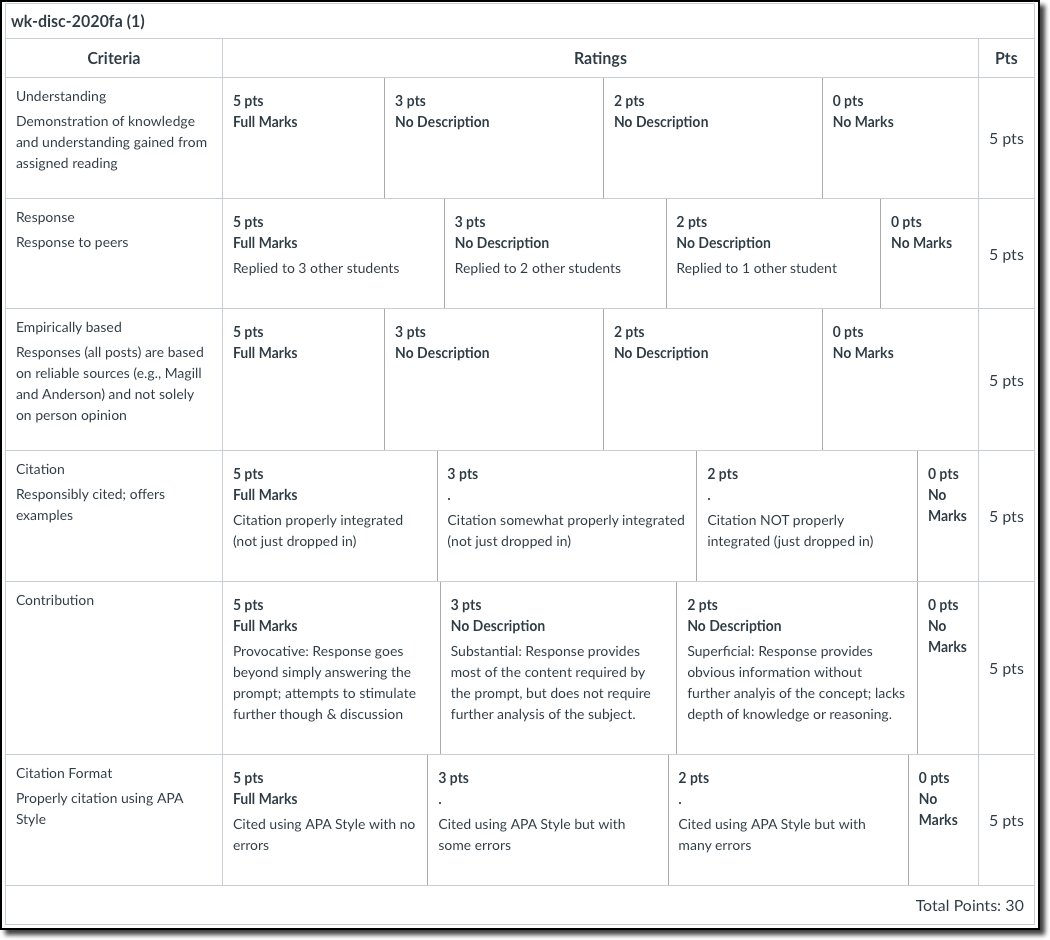
\includegraphics{images/paste-CCDC1445.png}

\hypertarget{final-performance---video}{%
\subsubsection{Final Performance -
Video}\label{final-performance---video}}

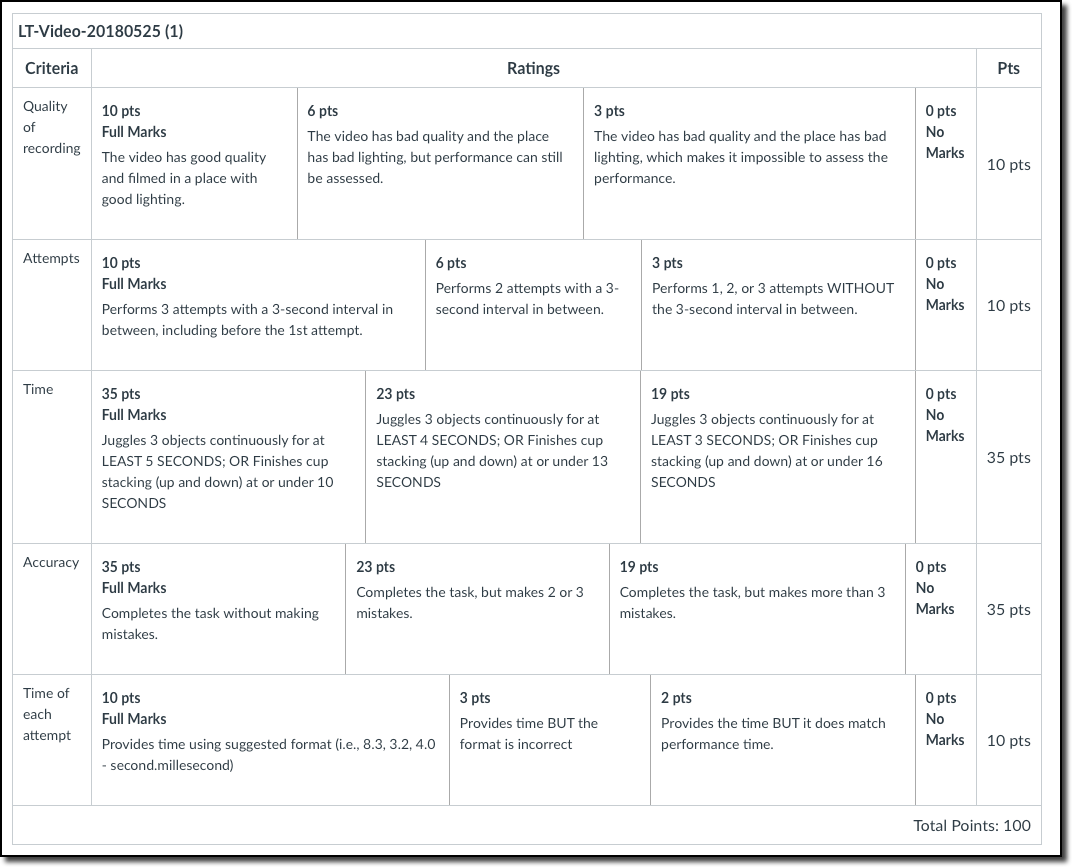
\includegraphics{images/paste-97AE7969.png}

\hypertarget{reflection-paper}{%
\subsubsection{Reflection Paper}\label{reflection-paper}}

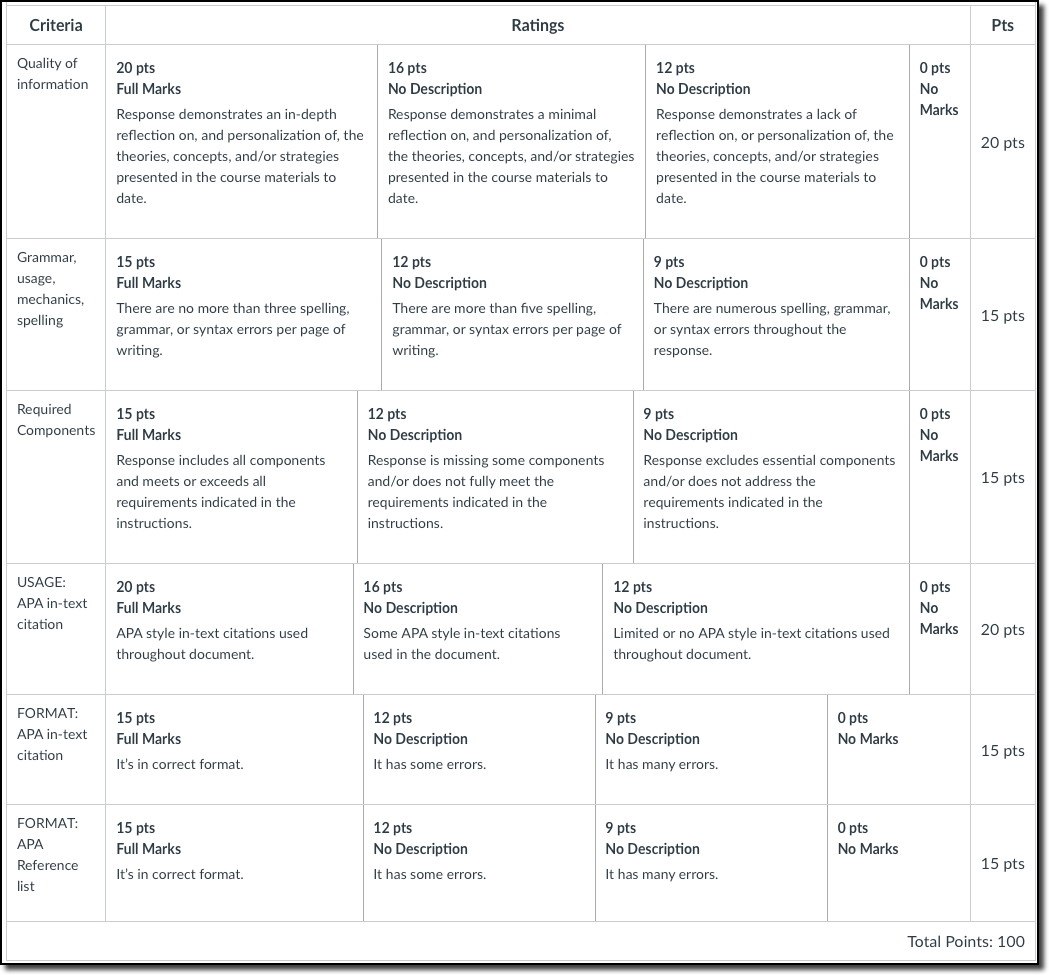
\includegraphics{images/paste-3AE7E91C.png}

\hypertarget{refs}{}
\begin{CSLReferences}{1}{0}
\leavevmode\vadjust pre{\hypertarget{ref-magill2020}{}}%
Magill, R. A., \& Anderson, D. (2020). \emph{Motor learning and control:
concepts and applications}. McGraw-Hill Education.
\url{https://www.bkstr.com/csunorthridgestore/product/motor-learning-and-control--concepts-and-applications-147614-1}

\end{CSLReferences}



\end{document}
